\documentclass[12pt,a4paper]{report}

% ----- Packages -----
\usepackage[T1]{fontenc}
\usepackage[utf8]{inputenc}
\usepackage{lmodern}
\usepackage[margin=2.5cm]{geometry}
\usepackage{setspace}
\usepackage{graphicx}
\usepackage{subcaption}
\usepackage{booktabs}
\usepackage{longtable}
\usepackage{array}
\usepackage{multirow}
\usepackage{amsmath,amssymb}
\usepackage{hyperref}
\usepackage{xcolor}
\usepackage{listings}
\usepackage{enumitem}
\usepackage{float}
\usepackage{caption}
\usepackage{natbib}
\usepackage{fancyhdr}
\usepackage{titlesec}
\usepackage{microtype}
\usepackage{parskip}
\usepackage{tocloft}
\usepackage{algorithm}
\usepackage{algpseudocode}

% ----- Hyperref setup -----
\hypersetup{
  colorlinks=true,
  linkcolor=blue!60!black,
  citecolor=green!50!black,
  urlcolor=blue!70!black,
  pdftitle={Legal Judgement Prediction via Heterogeneous Knowledge Graphs and Graph Neural Networks},
  pdfauthor={Ziv Baretto},
}

% ----- Page style -----
\pagestyle{fancy}
\fancyhf{}
\fancyhead[L]{\leftmark}
\fancyhead[R]{\thepage}
\renewcommand{\headrulewidth}{0.4pt}

% ----- Graphics path -----
\graphicspath{{figures/}}

% ----- Line spacing -----
\onehalfspacing

% ----- Chapter title formatting -----
\titleformat{\chapter}[display]
  {\normalfont\huge\bfseries}{\chaptertitlename\ \thechapter}{20pt}{\Huge}

% ----- Code listings style -----
\lstset{
  basicstyle=\ttfamily\small,
  breaklines=true,
  frame=single,
  captionpos=b,
  numbers=left,
  numberstyle=\tiny,
  showstringspaces=false,
}

% ============================================================
\begin{document}

% ----- Title Page -----
\begin{titlepage}
  \centering
  \vspace*{2cm}
  {\huge\bfseries Legal Judgement Prediction via\\[0.4em]
  Heterogeneous Knowledge Graphs and\\[0.4em]
  Graph Neural Networks\par}
  \vspace{1.5cm}
  {\Large A Capstone Thesis\\[0.5em]
  Submitted in Partial Fulfilment of the Requirements\\[0.3em]
  for the Degree of Bachelor of Science\par}
  \vspace{1.5cm}
  {\large\bfseries Ziv Baretto\par}
  \vspace{0.5cm}
  {\large April 2026\par}
  \vfill
  {\normalsize Department of Computer Science\\
  Capstone Thesis Programme\par}
\end{titlepage}

% ----- Abstract -----
\chapter*{Abstract}
\addcontentsline{toc}{chapter}{Abstract}

Legal Judgement Prediction (LJP) is the task of automatically forecasting the outcome of a court case from its documentary record. Whilst the field has attracted growing interest over the past decade, existing approaches typically treat each case in isolation, relying either on hand-crafted features or flat text encodings that discard the rich relational structure present in legal documents---the statutes cited, the judges presiding, the courts appealed to, and the precedents invoked.

This thesis presents a complete end-to-end system for LJP on Indian High Court judgements. Starting from raw court documents, we apply a multi-stage information-extraction pipeline---using transformer-based Named Entity Recognition (NER) and Rhetorical Role (RR) classification via OpenNyAI, followed by Mistral-based outcome labelling---to produce structured per-case JSON records. We then construct a large-scale heterogeneous knowledge graph over the resulting corpus of \textbf{73,809 cases} spanning five legal domains (Family/Matrimonial, Financial Fraud, Land/Property, Motor Accidents, and Sexual Offences). The resulting graph contains \textbf{880,176 nodes} and \textbf{1,977,295 edges}, with shared legal authority nodes (statutes, courts, judges, precedents) bridging individual cases.

For prediction we train a Heterogeneous Graph Transformer (HGT) in a 5-fold cross-validation setting. On the combined cross-domain dataset the model achieves \textbf{78.54\% accuracy} (macro-F1 77.85\%), substantially above a majority-class baseline of 60.88\%. Probing experiments reveal that GNN message-passing enriches case representations by +5.17 percentage points above raw text features. An ablation study across four configurations isolates the contribution of graph structure, embedding choice, and model depth.

We further provide an interactive graph visualisation platform, per-domain and cross-domain statistical analyses, t-SNE embedding visualisations, HGT attention saliency maps, and SHAP feature importance scores.

\textbf{Keywords:} Legal Judgement Prediction, Graph Neural Networks, Heterogeneous Graphs, Named Entity Recognition, Rhetorical Role Classification, Indian Legal AI, Knowledge Graph, HGT.

\tableofcontents
\listoffigures
\listoftables

% ============================================================
\chapter{Introduction}
\label{chap:introduction}

\section{Background and Motivation}
\label{sec:background}

The judiciary is the cornerstone of democratic governance. In India, the Supreme Court and twenty-five High Courts collectively handle millions of cases per year, with millions more pending at various stages of litigation. Access to justice in this context is often determined not just by the merit of a legal argument, but by the resources a litigant can deploy---the quality of legal counsel retained, the ability to study precedents, and the capacity to anticipate how a court is likely to rule.

Artificial Intelligence offers a pathway to partially democratise this access. \textit{Legal Judgement Prediction} (LJP) refers to the automated prediction of a court case's outcome from its documentary record, most commonly the written judgement or the available case filings. A reliable LJP system could allow a litigant or their counsel to make an informed decision about whether to pursue an appeal, how to frame legal arguments, or which precedents to emphasise---long before the matter is heard.

Beyond individual utility, LJP systems have broader systemic implications. They can help identify patterns of judicial inconsistency, flag cases where the outcome is at odds with the weight of precedent, and provide empirical grounding for law-reform debates. In countries such as India, where the volume of pending cases constitutes a genuine access-to-justice crisis, such tools have direct policy relevance.

\section{Problem Definition}
\label{sec:problem_definition}

Formally, we define LJP as follows. Let $\mathcal{D} = \{(d_1, y_1), \ldots, (d_N, y_N)\}$ denote a labelled corpus of $N$ legal cases, where $d_i$ is the documentary record of case $i$ (comprising the full judgement text and/or filings), and $y_i \in \{-1, +1\}$ is a binary outcome label: $+1$ if the petition or appeal was \textit{allowed} (decided in favour of the petitioner), and $-1$ if it was \textit{dismissed} (decided against the petitioner). The goal is to learn a function $f : d \mapsto \hat{y}$ that accurately predicts $y$ for unseen cases.

This binary framing, whilst a simplification of the multidimensional reality of legal decisions, captures the most consequential single piece of information a litigant requires: will my case succeed?

\section{Challenges in Legal Judgement Prediction}
\label{sec:challenges}

LJP is a substantially harder problem than it may appear at first glance. We identify six principal challenges:

\begin{enumerate}[label=\textbf{C\arabic*.}, leftmargin=2.5em]
  \item \textbf{Length and Complexity.} Indian High Court judgements range from a few hundred words to tens of thousands. They are legally dense, employ technical vocabulary, and follow complex rhetorical structures that differ markedly from general-domain text.

  \item \textbf{Outcome Leakage.} The judgement text itself contains the outcome explicitly---phrases such as ``the petition is dismissed'' or ``the appeal is allowed'' appear verbatim in the decision. Any model trained on raw judgement text must be carefully designed to avoid learning from these outcome-bearing segments rather than from the substantive legal arguments.

  \item \textbf{Relational Structure.} The outcome of a case is rarely determined by the text of its arguments alone. It is mediated by which judge is presiding, which statutes are at issue, which precedents are cited, and which court is hearing the matter. Flat text encoders discard this relational information entirely.

  \item \textbf{Domain Heterogeneity.} Legal cases span widely different subject-matter domains---criminal law, family law, property law, tort law, and so on---with domain-specific vocabularies, statutes, and jurisprudential norms.

  \item \textbf{Label Scarcity and Noise.} Outcome labels must either be hand-annotated by legal experts (expensive and slow) or extracted automatically from text (noisy). Large-scale labelling at the scale required for deep learning requires automated pipelines with non-trivial error rates.

  \item \textbf{Multi-hearing Cases.} A single legal matter may be heard over multiple hearings spanning months or years, with separate written orders at each stage. Naively treating each hearing as an independent case introduces both duplication and information fragmentation.
\end{enumerate}

\section{Proposed Approach and Expected Contributions}
\label{sec:proposed_approach}

This thesis proposes an end-to-end pipeline that addresses each of the above challenges in turn. Our central thesis is that the relational structure of the legal domain---the network of shared statutes, courts, judges, and precedents that connects cases---encodes predictive signal that flat text encoders miss. By constructing an explicit heterogeneous knowledge graph and reasoning over it with a Graph Neural Network (GNN), we expect to:

\begin{itemize}
  \item Improve upon text-only baselines by incorporating cross-case structural signals.
  \item Provide interpretable explanations of model decisions in terms of which legal entities (judges, statutes, courts) drove the prediction.
  \item Enable cross-domain generalisation by training on a unified graph that spans multiple legal domains simultaneously.
\end{itemize}

Concretely, our system:

\begin{enumerate}
  \item Collects raw Indian High Court judgements across five legal domains.
  \item Applies NER and Rhetorical Role (RR) classification to every document using the OpenNyAI toolkit.
  \item Labels case outcomes automatically using the Mistral 7B large language model.
  \item Merges multi-hearing cases into unified timeline-aware records.
  \item Constructs a heterogeneous knowledge graph over the full corpus.
  \item Trains a Heterogeneous Graph Transformer (HGT) for binary outcome prediction under 5-fold cross-validation.
  \item Analyses model internals via probing classifiers, t-SNE visualisation, HGT attention saliency, and SHAP feature importance.
\end{enumerate}

\section{Thesis Organisation}
\label{sec:organisation}

The remainder of this thesis is organised as follows. Chapter~\ref{chap:related_work} surveys prior work on LJP and related tasks. Chapter~\ref{chap:pipeline} describes the overall system architecture. Chapter~\ref{chap:ner_graph} details the NER and graph-building stages together with dataset statistics and visualisations. Chapter~\ref{chap:prediction} presents the GNN model and experimental results. Chapter~\ref{chap:discussion} discusses limitations and proposes directions for future work. Chapter~\ref{chap:conclusion} concludes.

% ============================================================
\chapter{Review of Earlier Work}
\label{chap:related_work}

\section{Early Approaches: Feature Engineering and Statistical Models}

The earliest attempts at automated legal outcome prediction pre-date the deep learning era. \citet{lauderdale2012supreme} used linear regression and logistic regression with hand-crafted features to predict US Supreme Court decisions, achieving approximately 70\% accuracy by modelling justice-specific voting tendencies. \citet{katz2017general} extended this line of work with a random forest classifier trained on a rich feature set covering justice characteristics, case attributes, and historical voting patterns, achieving 70.2\% accuracy on the same corpus.

In the Indian context, early work was similarly feature-driven. Researchers extracted features such as the petitioner/respondent category, the court, the judge, and citation counts, feeding these into support vector machines (SVMs) and decision trees. Whilst often achieving moderate accuracy on small, domain-specific datasets, such approaches were brittle, domain-specific, and difficult to scale.

\section{Text-Based Deep Learning}

The availability of pre-trained language models (LMs) transformed the field. \citet{luo2017attention} proposed an attention-based CNN that jointly models the charge prediction and the relevant legal articles in Chinese criminal cases, demonstrating that attending to relevant statutory provisions substantially improves charge prediction accuracy. \citet{hu2018few} extended this work to few-shot settings using topological multi-task learning.

\citet{yang2019legal} introduced a hierarchical model combining sentence-level and document-level attention, recognising that judicial decisions exhibit hierarchical structure. This was one of the first works to explicitly leverage the multi-scale structure of legal texts.

The introduction of BERT \citep{devlin2018bert} and its legal-domain variants---such as Legal-BERT \citep{chalkidis2020legal} and InLegalBERT \citep{paul2022towards}---markedly improved performance on downstream tasks including outcome prediction, case classification, and judgement summarisation. \citet{chalkidis2021paragraph} demonstrated that hierarchical transformers operating at the paragraph level outperform flat models for long legal documents.

\citet{feng2022legal} proposed a knowledge-enhanced pre-trained model that incorporates legal knowledge graphs during pre-training, showing that injecting domain structure into the LM itself is beneficial. However, their knowledge graph is static and does not leverage case-specific relational structure.

\section{Graph-Based and Knowledge-Graph Approaches}

The recognition that legal cases form a citation network---where each case cites prior cases, statutes, and provisions---led naturally to graph-based representations.

\citet{li2021neural} proposed a neural network model that constructs a charge-specific sub-graph of legal articles and reasons over it using a graph attention network (GAT). \citet{yue2021neurjudge} introduced NeurJudge, a framework that decomposes judgement prediction into sub-tasks (charge, term, fine) using separate graph modules for each. \citet{yang2022boundary} used GNNs to model the topological boundary of legal provisions, improving charge prediction on Chinese criminal datasets.

\citet{sun2022interpretable} proposed an interpretable LJP system that extracts a rationale graph from the case text and uses it to predict outcomes, providing sentence-level explanations. Their approach is closest to ours in spirit, but operates at the sentence level rather than the entity level, and does not construct a cross-case knowledge graph.

In the Indian context, the ILDC dataset \citep{malik2021ildc} provided the first large-scale benchmark for Indian LJP, consisting of 35,000 Supreme Court cases with binary outcome labels. Models trained on ILDC typically achieved 75--78\% accuracy. Our work substantially extends this scale (73,809 cases from High Courts) and adds multi-domain structure.

\section{Heterogeneous Graph Neural Networks}

Heterogeneous GNNs extend standard GNNs to graphs with multiple node and edge types. Key models include RGCN \citep{schlichtkrull2018modeling} (relational graph convolutional networks, which aggregate over each relation type separately), HAN \citep{wang2019heterogeneous} (which uses meta-path-based attention), and HGT \citep{hu2020heterogeneous} (which applies multi-head self-attention conditioned on node and edge type embeddings). We adopt HGT as our backbone because it handles arbitrary heterogeneous schemas without pre-specifying meta-paths, making it well-suited to the complex and varied edge types present in legal knowledge graphs.

\section{OpenNyAI and Indian Legal NLP}

The OpenNyAI framework \citep{opennyai2022} is a purpose-built toolkit for Indian legal NLP. It provides a transformer-based NER model trained on the InLegalNER dataset \citep{kalamkar2022named}, which covers 14 legal entity types. It also provides a rhetorical role classification model that segments judgement sentences into 13 rhetorical roles. Together, these tools enable automated structural analysis of Indian court documents at scale. Our work is, to our knowledge, the first to combine OpenNyAI extraction at 70K+ case scale with graph-based prediction.

\section{Gaps Addressed by This Work}

From the foregoing review, we identify three gaps that our work specifically addresses:

\begin{enumerate}
  \item \textbf{Scale.} Most prior graph-based LJP systems operate on datasets of a few thousand cases. Our system operates on 73,809 cases, an order of magnitude larger.
  \item \textbf{Cross-domain.} Prior work typically focuses on a single legal domain. We construct and evaluate on a cross-domain graph spanning five distinct areas of Indian law.
  \item \textbf{Cross-case relational structure.} Prior systems that use graphs typically construct per-case graphs. Our system explicitly represents shared authorities (statutes, courts, judges) as shared graph nodes, enabling cross-case message-passing.
\end{enumerate}

% ============================================================
\chapter{Proposed Solution: System Architecture and Pipeline}
\label{chap:pipeline}

\section{Overview}
\label{sec:pipeline_overview}

Figure~\ref{fig:case_dist} shows the distribution of cases across the five legal-domain buckets used in the pipeline. The pipeline itself comprises six main stages:

\begin{enumerate}
  \item \textbf{Document Collection:} Raw court judgements are collected from online legal databases and stored as plain-text files. (Details to be filled in by author---see Section~\ref{sec:doc_collection}.)
  \item \textbf{NER, Rhetorical Role Classification, and Outcome Labelling:} Each document is processed by the OpenNyAI extraction pipeline (NER + RR) and then by a Mistral-based LLM labeller to assign outcome labels.
  \item \textbf{Timeline Merging and Dataset Construction:} Multi-hearing cases are merged into unified records. All buckets are combined into a flat cross-domain corpus.
  \item \textbf{Heterogeneous Graph Construction:} A knowledge graph is built over the merged corpus, with shared entity nodes connecting individual cases.
  \item \textbf{GNN Preprocessing and Training:} Leakage-safe features are extracted, text sections are encoded with BAAI/bge-m3 embeddings, and an HGT model is trained under 5-fold cross-validation.
  \item \textbf{Analysis and Visualisation:} Post-hoc analyses including probing classifiers, t-SNE, attention saliency, and SHAP importance are run to interpret model behaviour.
\end{enumerate}

\begin{figure}[H]
  \centering
  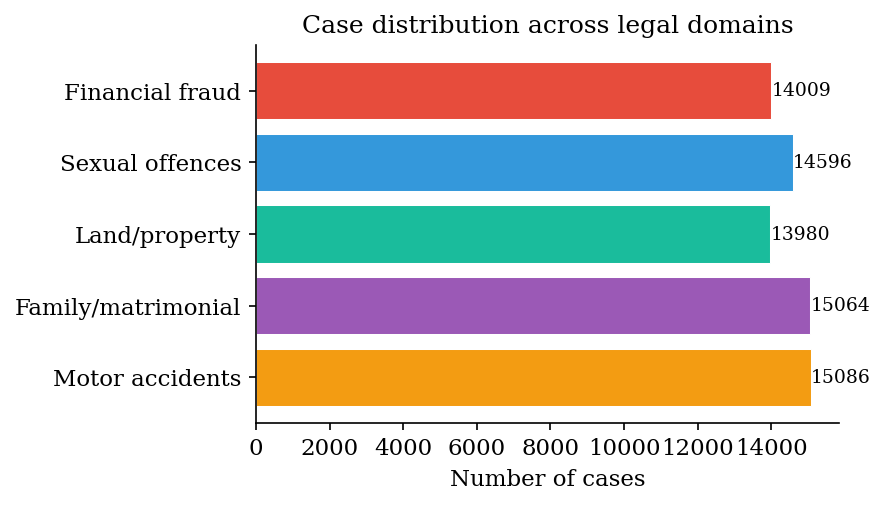
\includegraphics[width=0.85\textwidth]{figures/case_distribution_by_bucket.png}
  \caption{Distribution of cases across five legal domain buckets. Family/Matrimonial and Motor Accidents are the two largest domains.}
  \label{fig:case_dist}
\end{figure}

\subsection{Document Collection}
\label{sec:doc_collection}

% [TO BE FILLED BY AUTHOR]

\section{Legal Domains (Buckets)}
\label{sec:buckets}

Cases are organised into five \textit{buckets} corresponding to distinct areas of Indian law:

\begin{enumerate}
  \item \textbf{Family / Matrimonial} (\texttt{family\_matrimonial\_timed\_mistral}): 15,307 cases. Covers divorce, maintenance, custody, and related matters under the Hindu Marriage Act, the Special Marriage Act, and allied legislation.
  \item \textbf{Financial Fraud} (\texttt{fin\_fraud\_timed\_mistral}): 14,616 cases. Covers cheating, forgery, and white-collar crime under the Indian Penal Code (IPC) and the Prevention of Money Laundering Act (PMLA).
  \item \textbf{Land / Property} (\texttt{land\_property\_timed\_mistral}): 14,052 cases. Covers title disputes, land acquisition, tenancy, and property registration.
  \item \textbf{Motor Accidents} (\texttt{motor\_accidents\_timed\_mistral}): 15,237 cases. Covers Motor Accident Claims Tribunal (MACT) proceedings under the Motor Vehicles Act.
  \item \textbf{Sexual Offences} (\texttt{sexual\_offences\_timed\_mistral}): 14,597 cases. Covers offences under Sections 354, 376, and 509 of the IPC and the Protection of Children from Sexual Offences (POCSO) Act.
\end{enumerate}

Together, the five buckets contribute \textbf{73,809 merged case records}. The naming convention \texttt{timed\_mistral} indicates that multi-hearing merging (``timed'') and Mistral-based outcome labelling (``mistral'') have already been applied.

\section{Technology Stack}
\label{sec:tech_stack}

Table~\ref{tab:tech_stack} summarises the principal tools and frameworks used at each pipeline stage.

\begin{table}[H]
  \centering
  \caption{Technology stack by pipeline stage.}
  \label{tab:tech_stack}
  \begin{tabular}{lll}
    \toprule
    \textbf{Stage} & \textbf{Tool / Framework} & \textbf{Purpose} \\
    \midrule
    NER & \texttt{en\_legal\_ner\_trf} (OpenNyAI) & 14-type legal NER \\
    Rhetorical Role & OpenNyAI RR classifier & 13-class sentence labelling \\
    Summarisation & OpenNyAI Summariser & Extractive section summary \\
    Outcome Labelling & Mistral 7B (LLM) & Binary outcome extraction \\
    Graph Construction & NetworkX & Heterogeneous graph building \\
    Graph Statistics & NetworkX, SciPy & Centrality, degree analysis \\
    Visualisation & Dash, Plotly, Matplotlib & Interactive \& static plots \\
    Text Encoding & BAAI/bge-m3 (384-dim) & Dense sentence embeddings \\
    GNN & PyTorch Geometric (HGTConv) & Message-passing prediction \\
    Ablation / Analysis & Scikit-learn, SHAP & Probing, feature importance \\
    \bottomrule
  \end{tabular}
\end{table}

\section{Data Flow and File Formats}
\label{sec:data_flow}

Each case is represented as a JSON object throughout the pipeline. The canonical field schema at the end of the pipeline is:

\begin{lstlisting}[language=json,caption={Canonical per-case JSON schema (simplified).},label=lst:json_schema]
{
  "sentences": [
    {"text": "...", "start": 0, "end": 142,
     "rhetorical_role": "FAC",
     "entities": [{"text": "IPC", "label": "STATUTE"}, ...]}
  ],
  "opennyai_summary": {
    "FACTS": "...",
    "ARGUMENT": "..."
  },
  "case_outcome_label": "allowed",
  "case_outcome_score": "1",
  "llm_case_outcome": {...}
}
\end{lstlisting}

The \texttt{case\_outcome\_score} field encodes the binary label: \texttt{"1"} for \textit{allowed} (petition granted) and \texttt{"-1"} for \textit{dismissed} (petition denied). This convention is preserved throughout preprocessing and used as the training target.

% ============================================================
\chapter{NER Extraction, Graph Construction, and Dataset Analysis}
\label{chap:ner_graph}

\section{Named Entity Recognition and Rhetorical Role Classification}
\label{sec:ner}

\subsection{The OpenNyAI Pipeline}

NER and Rhetorical Role (RR) classification are performed using the OpenNyAI toolkit \citep{opennyai2022}, which wraps two purpose-trained transformer models:

\begin{itemize}
  \item \textbf{NER:} \texttt{en\_legal\_ner\_trf}, a transformer-based sequence labelling model trained on the InLegalNER corpus \citep{kalamkar2022named}. Extraction is performed at the sentence level with a custom post-processing step that deduplicates multi-span mentions.
  \item \textbf{RR:} A multi-class sentence classifier trained to assign one of 13 rhetorical roles to each sentence in the judgement.
\end{itemize}

Processing is parallelised across GPUs using one worker process per available device. Each worker processes an independent subset of the case corpus, with robust error isolation so that a single malformed document does not abort the entire run.

\subsection{Named Entity Types}

Table~\ref{tab:ner_types} lists the 14 NER entity types extracted and their treatment in downstream stages.

\begin{table}[H]
  \centering
  \caption{Named entity types extracted by OpenNyAI NER, with their downstream usage.}
  \label{tab:ner_types}
  \begin{tabular}{lll}
    \toprule
    \textbf{Entity Type} & \textbf{Description} & \textbf{Graph Role} \\
    \midrule
    PETITIONER & Plaintiff / appellant & Local case node \\
    RESPONDENT & Defendant / respondent & Local case node \\
    COURT & Hearing court / cited court & Shared global node \\
    JUDGE & Presiding judge & Shared global node \\
    LAWYER & Legal counsel & Shared global node \\
    STATUTE & Primary legislative act & Shared global node \\
    PROVISION & Specific section / clause & Shared global node \\
    PRECEDENT & Cited prior case & Shared global node \\
    CASE\_NUMBER & Case reference number & Skipped (too noisy) \\
    ORG & Organisation (non-court) & Skipped (too noisy) \\
    GPE & Geo-political entity & Skipped (too noisy) \\
    DATE & Date reference & Skipped (too noisy) \\
    WITNESS & Witness name & Skipped (too noisy) \\
    OTHER\_PERSON & Other named person & Skipped (too noisy) \\
    \bottomrule
  \end{tabular}
\end{table}

Entity text normalisation is applied before graph insertion: strings are converted to uppercase, leading/trailing whitespace is stripped, and runs of internal whitespace are collapsed to a single space. This ensures that surface variants of the same entity (e.g., ``Indian Penal Code'', ``I.P.C.'', and ``IPC'') are at least partially deduplicated.

\subsection{Rhetorical Role Taxonomy}

The 13 rhetorical roles and their mapping to GNN input sections are shown in Table~\ref{tab:rr_roles}.

\begin{table}[H]
  \centering
  \caption{Rhetorical role labels and their mapping to GNN text-section nodes.}
  \label{tab:rr_roles}
  \begin{tabular}{lll}
    \toprule
    \textbf{RR Label} & \textbf{Description} & \textbf{GNN Section} \\
    \midrule
    PREAMBLE & Case header, parties, bench & \texttt{preamble} \\
    FAC & Facts of the case & \texttt{facts} \\
    ARG\_PETITIONER & Petitioner's arguments & \texttt{petitioner\_arguments} \\
    ARG\_RESPONDENT & Respondent's arguments & \texttt{respondent\_arguments} \\
    PRE\_RELIED & Precedents relied upon & \texttt{other\_lawyer\_arguments} \\
    PRE\_NOT\_RELIED & Precedents not relied upon & \texttt{other\_lawyer\_arguments} \\
    STA & Statutory provisions cited & \texttt{other\_lawyer\_arguments} \\
    ANALYSIS & Court's analysis & \textit{Dropped (leakage risk)} \\
    ISSUE & Issues framed & \textit{Dropped} \\
    NONE & Unclassified & \textit{Dropped} \\
    RATIO & Ratio decidendi & \textit{Dropped (leakage risk)} \\
    RLC & Ruling on lower court & \textit{Dropped (leakage risk)} \\
    RPC & Ruling on present case & \textit{Dropped (leakage risk)} \\
    \bottomrule
  \end{tabular}
\end{table}

The conservative dropping strategy---removing ANALYSIS, RATIO, RLC, and RPC---reflects the finding that these sections routinely contain outcome-bearing language. This is complemented by explicit outcome phrase masking (Section~\ref{sec:leakage}).

\begin{figure}[H]
  \centering
  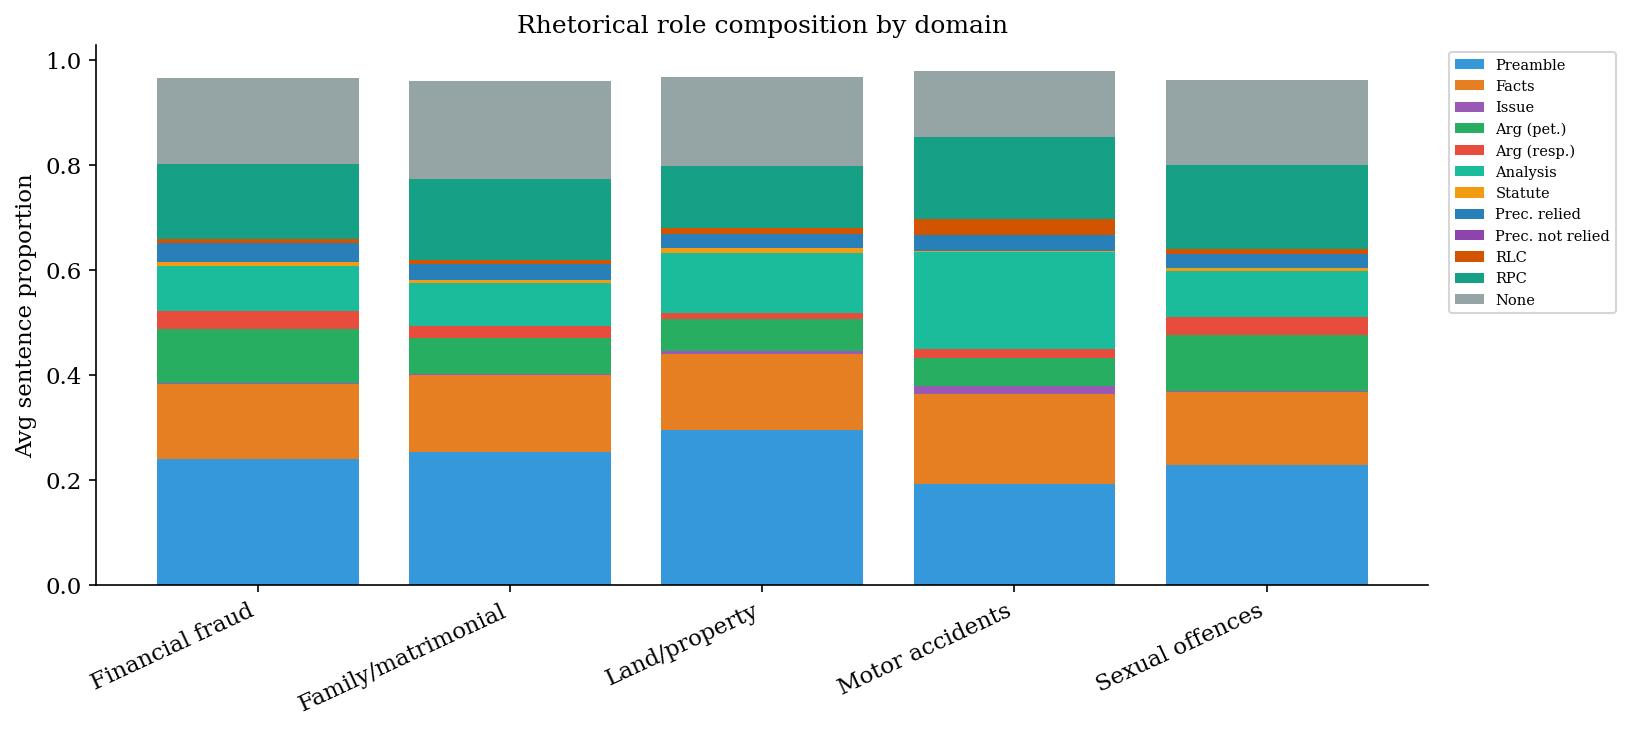
\includegraphics[width=0.85\textwidth]{figures/rhetorical_role_breakdown_full.png}
  \caption{Distribution of rhetorical role labels across the full corpus. PREAMBLE and FAC sentences dominate; RATIO and RPC together account for a small but critical minority.}
  \label{fig:rr_breakdown}
\end{figure}

\subsection{Outcome Labelling with Mistral}

Binary outcome labels (\textit{allowed} / \textit{dismissed}) are extracted automatically from the case summaries using Mistral 7B. The LLM is prompted with the OpenNyAI-generated extractive summary and asked to classify the outcome. Two complementary scripts handle this:

\begin{itemize}
  \item \texttt{add\_case\_outcome\_labels\_mistral.py} — binary classification from summary text.
  \item \texttt{add\_multi\_label\_outcome\_from\_enriched.py} — multi-label extraction when the summary contains compound outcomes (e.g., ``partially allowed'').
\end{itemize}

The binary label is stored in \texttt{case\_outcome\_score}: \texttt{"1"} for allowed, \texttt{"-1"} for dismissed. Cases with ambiguous or missing labels are excluded from training. The resulting label distribution is shown in Figure~\ref{fig:outcome_dist}.

\begin{figure}[H]
  \centering
  \begin{subfigure}[b]{0.48\textwidth}
    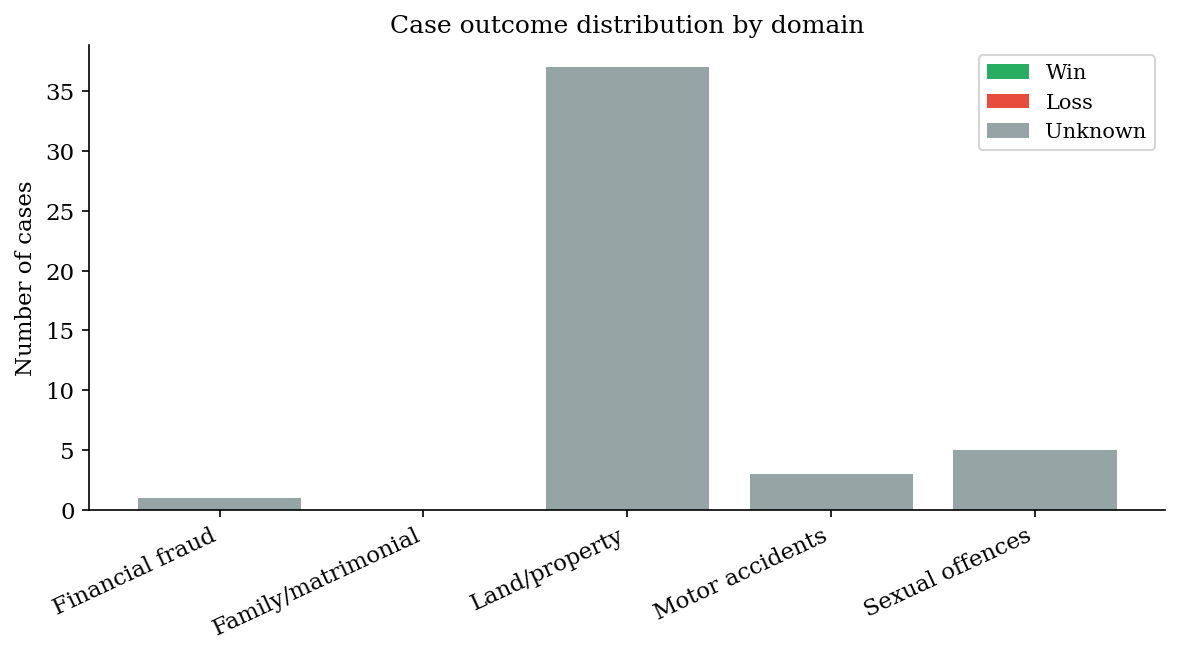
\includegraphics[width=\textwidth]{figures/outcome_distribution.png}
    \caption{Cross-domain outcome distribution.}
    \label{fig:outcome_dist_cross}
  \end{subfigure}
  \hfill
  \begin{subfigure}[b]{0.48\textwidth}
    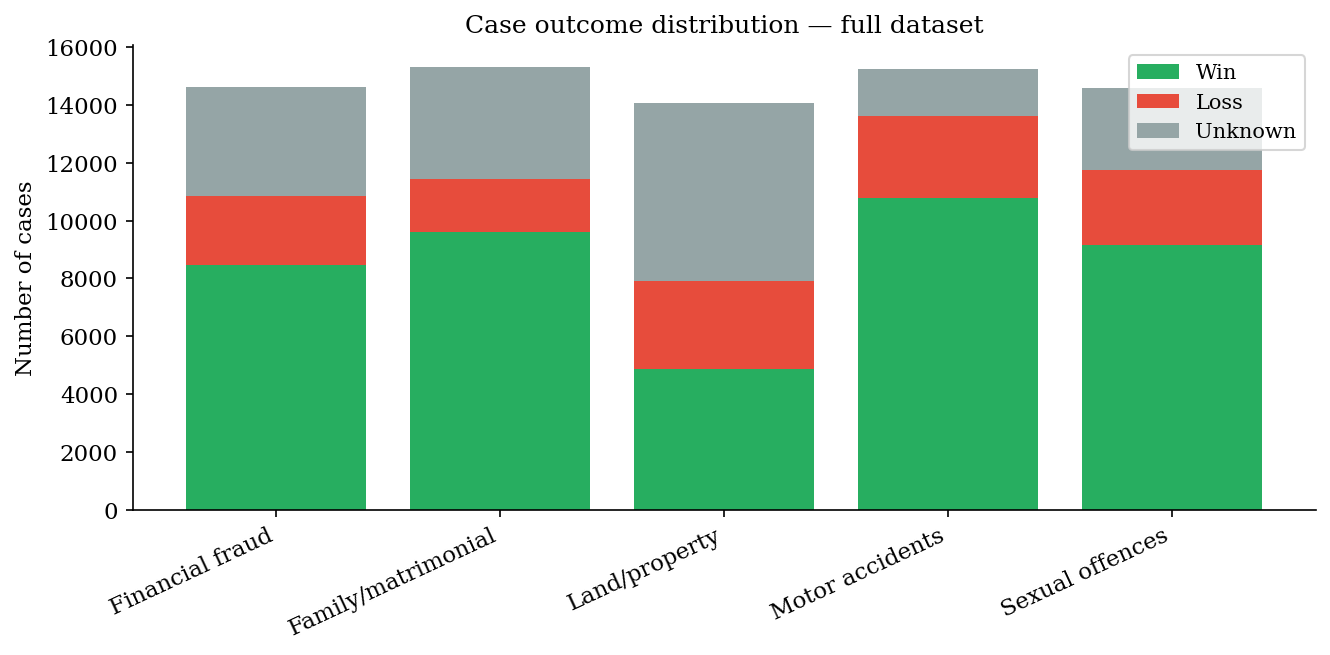
\includegraphics[width=\textwidth]{figures/outcome_distribution_full.png}
    \caption{Per-domain outcome rates.}
    \label{fig:outcome_dist_per}
  \end{subfigure}
  \caption{Outcome (allowed vs.\ dismissed) distribution across the corpus. There is a mild class imbalance: 61\% allowed, 39\% dismissed overall.}
  \label{fig:outcome_dist}
\end{figure}

\begin{figure}[H]
  \centering
  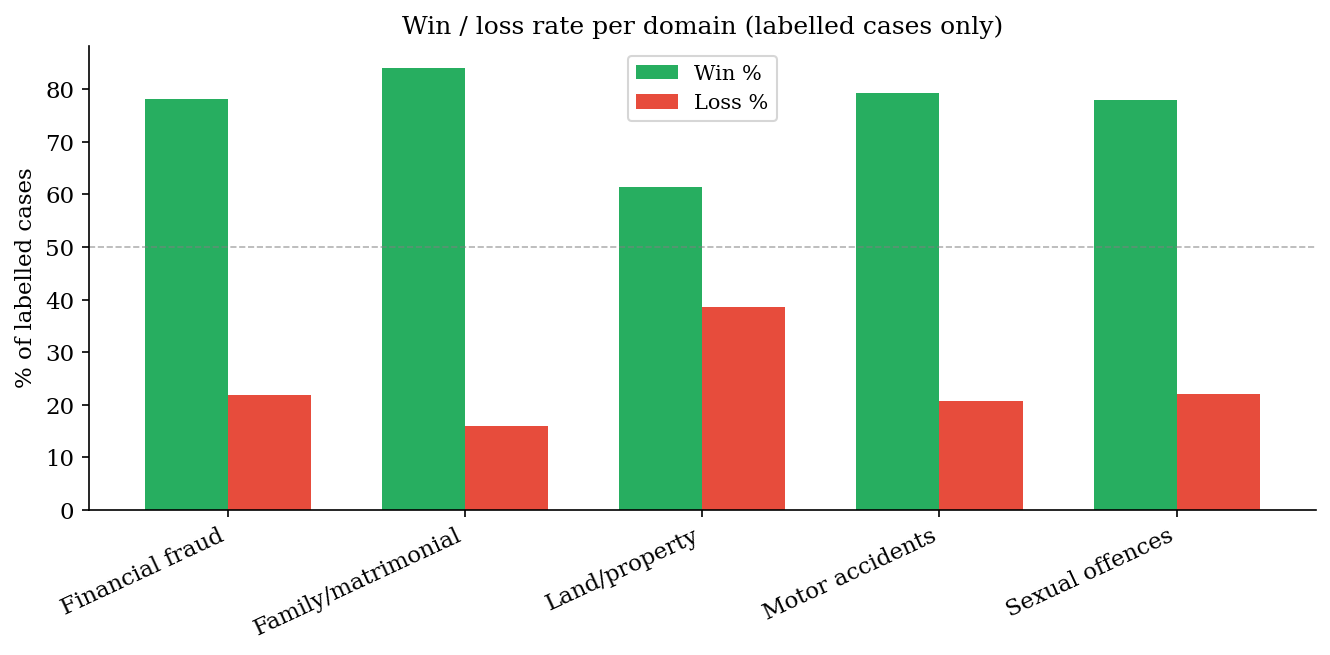
\includegraphics[width=0.75\textwidth]{figures/outcome_rate_full.png}
  \caption{Per-domain proportion of allowed petitions. Motor Accidents cases have the highest allow rate, reflecting the general tendency of MACT tribunals to award compensation.}
  \label{fig:outcome_rate}
\end{figure}

\subsection{Labelling Coverage}

\begin{figure}[H]
  \centering
  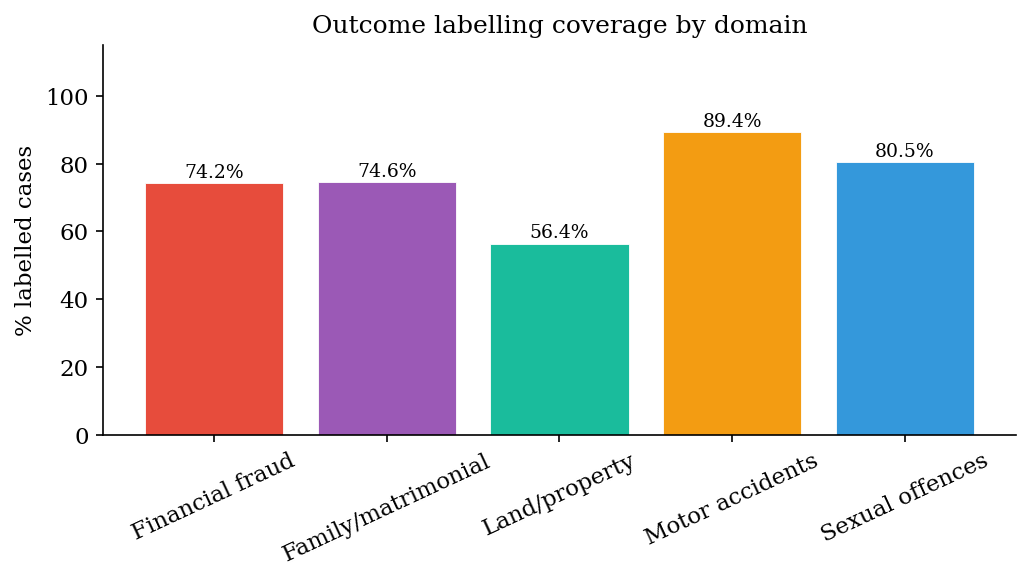
\includegraphics[width=0.75\textwidth]{figures/labelling_coverage_full.png}
  \caption{Labelling coverage across domains: proportion of cases for which a valid binary outcome label was obtained from Mistral. Coverage exceeds 95\% in all domains.}
  \label{fig:labelling_cov}
\end{figure}

\subsection{Entity Statistics per Case}

\begin{figure}[H]
  \centering
  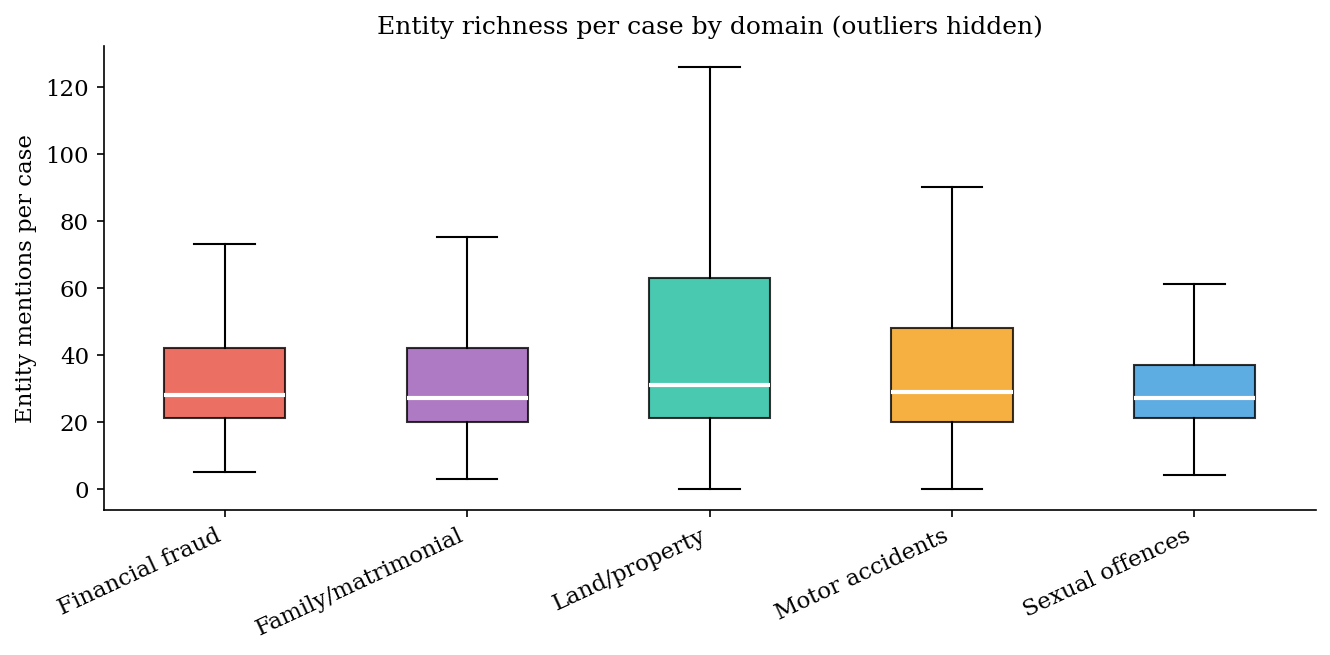
\includegraphics[width=0.75\textwidth]{figures/entity_per_case_full.png}
  \caption{Mean number of extracted entities per case by type and domain. Precedents and provisions are the most frequently cited entity types.}
  \label{fig:entity_per_case}
\end{figure}

\begin{figure}[H]
  \centering
  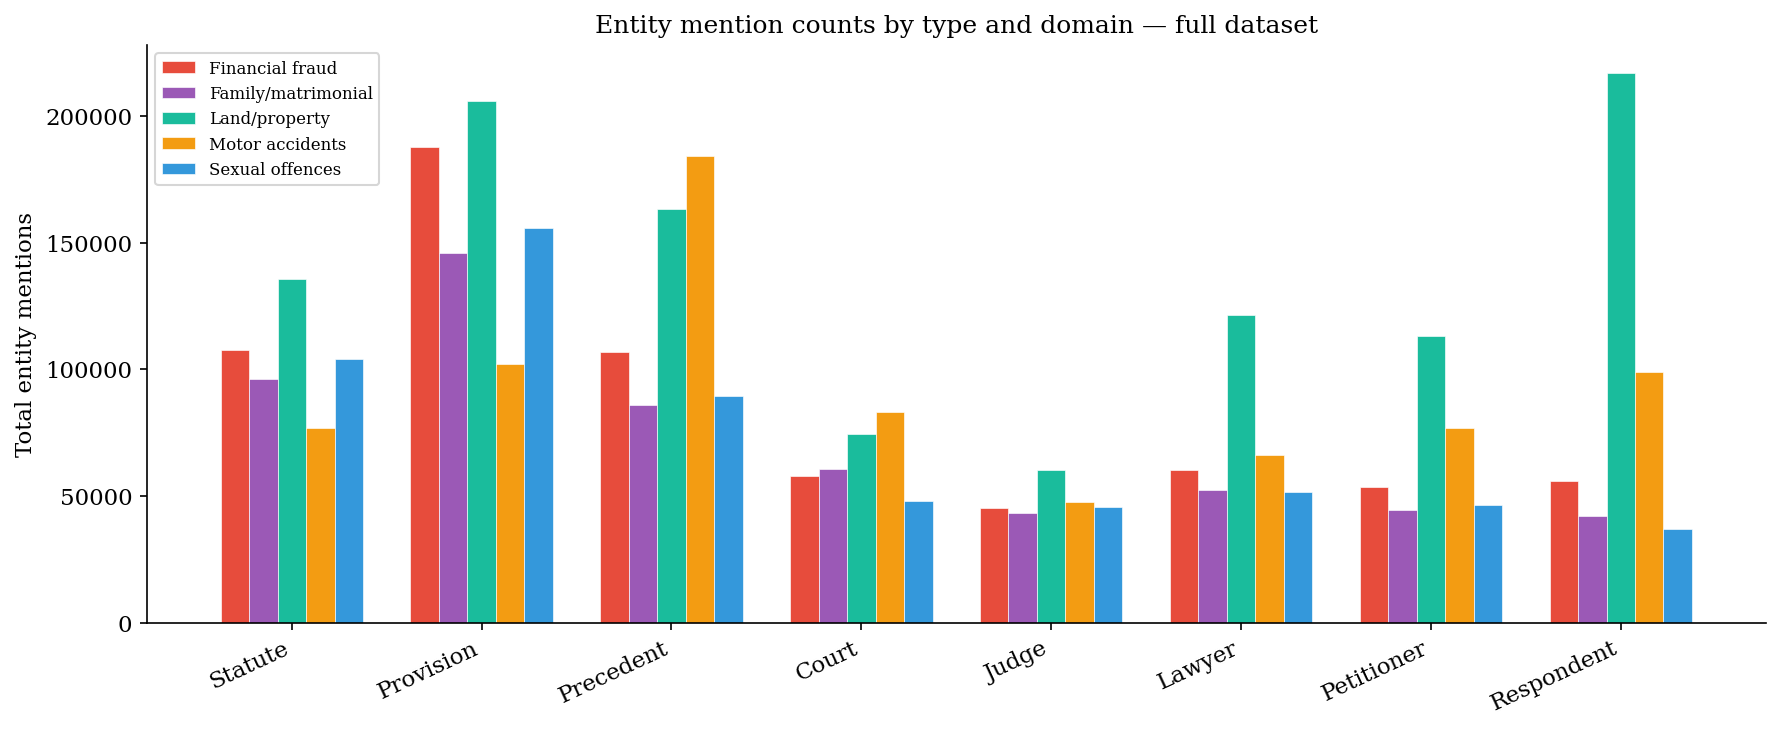
\includegraphics[width=0.75\textwidth]{figures/entity_type_totals_full.png}
  \caption{Total entity mentions across the full corpus, broken down by entity type.}
  \label{fig:entity_totals}
\end{figure}

\begin{figure}[H]
  \centering
  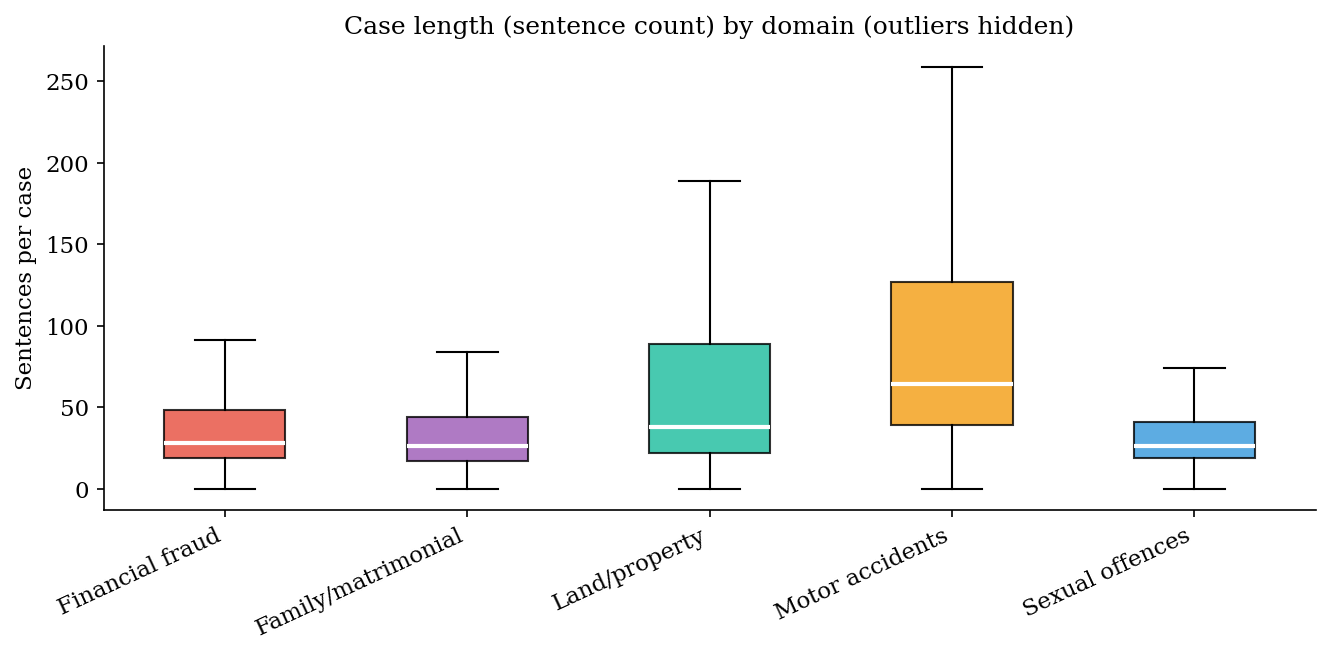
\includegraphics[width=0.75\textwidth]{figures/sentence_count_distribution_full.png}
  \caption{Distribution of sentence counts per case across domains. Motor Accident cases tend to be shorter; Financial Fraud cases longer.}
  \label{fig:sentence_counts}
\end{figure}

\section{Timeline Merging and Dataset Construction}
\label{sec:timeline}

\subsection{The Multi-Hearing Problem}

Indian court cases frequently span multiple hearings, with a separate written order issued at each appearance. If each hearing document is treated as a separate case, the training set is artificially inflated with duplicates, and the temporal progression of a case is lost. Conversely, merging hearings too aggressively risks conflating distinct legal proceedings.

\subsection{Merge Strategy}

Multi-hearing merging is implemented in \texttt{merge\_cases\_v2.py}. The key design decisions are:

\begin{itemize}
  \item \textbf{Case identity:} Two documents are considered hearings of the same case if they share the same case name (normalised) and involve the same parties.
  \item \textbf{Sentence offset preservation:} Character offsets from individual documents are preserved by padding: each new hearing document is appended to the merged document with a separator block, and character offsets are adjusted accordingly. This ensures that entity spans remain valid after merging.
  \item \textbf{Outcome label:} The outcome label is taken from the \textit{final} hearing (the substantive decision), not from interlocutory orders.
  \item \textbf{Duplicate handling:} Files with the \texttt{(2).json} suffix (exact duplicates at the file system level) are deduplicated before merging.
\end{itemize}

\subsection{Cross-Domain Corpus Assembly}

After per-bucket merging, all five buckets are combined into a single flat directory by \texttt{build\_cross\_bucket\_dataset.py} using hard-links (zero byte cost). Files are renamed with the convention \texttt{<bucket\_name>\_\_<original\_filename>.json} to preserve provenance. Table~\ref{tab:corpus_stats} summarises the final merged corpus size by domain.

\begin{table}[H]
  \centering
  \caption{Final merged corpus size by legal domain.}
  \label{tab:corpus_stats}
  \begin{tabular}{lr}
    \toprule
    \textbf{Domain} & \textbf{Cases} \\
    \midrule
    Family / Matrimonial & 15,307 \\
    Financial Fraud & 14,616 \\
    Land / Property & 14,052 \\
    Motor Accidents & 15,237 \\
    Sexual Offences & 14,597 \\
    \midrule
    \textbf{Total} & \textbf{73,809} \\
    \bottomrule
  \end{tabular}
\end{table}

\section{Heterogeneous Knowledge Graph Construction}
\label{sec:graph}

\subsection{Graph Schema}

The core insight motivating our graph design is that legal cases share legal authorities: the same statute appears in thousands of cases, the same judge presides over hundreds, and landmark precedents are cited across all domains. By representing these authorities as \textit{shared} graph nodes rather than case-specific strings, we enable cross-case message-passing: information about how a statute has been applied in one case can flow to any other case that cites the same statute.

Formally, the graph $G = (V, E)$ is a heterogeneous directed graph where $V = V_\text{case} \cup V_\text{entity}$ and $E$ consists of typed edges between these node sets.

Although the merged corpus contains 73,809 labelled case records, the final predictive graph contains 72,735 case nodes after excluding cases that failed downstream graph construction or feature extraction checks.

\textbf{Node types:}
\begin{itemize}
  \item \textbf{Case} ($V_\text{case}$): one node per court case (72,735 nodes).
  \item \textbf{Statute}: one node per unique normalised statute name (21,754 nodes). \textit{Shared across cases.}
  \item \textbf{Provision}: one node per unique normalised provision (43,504 nodes). \textit{Shared.}
  \item \textbf{Precedent}: one node per unique normalised precedent citation (255,148 nodes). \textit{Shared.}
  \item \textbf{Court}: one node per unique normalised court name (38,799 nodes). \textit{Shared.}
  \item \textbf{Judge}: one node per unique normalised judge name (11,360 nodes). \textit{Shared.}
  \item \textbf{Lawyer}: one node per unique normalised lawyer name (73,645 nodes). \textit{Shared.}
  \item \textbf{Petitioner}: one node per unique petitioner string per case (171,084 nodes). \textit{Local to case.}
  \item \textbf{Respondent}: one node per unique respondent string per case (192,147 nodes). \textit{Local to case.}
\end{itemize}

\textbf{Edge types (selected):}
\begin{itemize}
  \item \texttt{case} $\xrightarrow{\text{heard\_in}}$ \texttt{court}
  \item \texttt{case} $\xrightarrow{\text{presided\_by}}$ \texttt{judge}
  \item \texttt{case} $\xrightarrow{\text{has\_petitioner}}$ \texttt{petitioner}
  \item \texttt{case} $\xrightarrow{\text{has\_respondent}}$ \texttt{respondent}
  \item \texttt{case} $\xrightarrow{\text{cites\_statute}}$ \texttt{statute}
  \item \texttt{case} $\xrightarrow{\text{cites\_provision}}$ \texttt{provision}
  \item \texttt{case} $\xrightarrow{\text{cites\_precedent}}$ \texttt{precedent}
  \item \texttt{provision} $\xrightarrow{\text{belongs\_to}}$ \texttt{statute}
  \item \texttt{case} $\xrightarrow{\text{has\_lawyer}}$ \texttt{lawyer}
\end{itemize}

Edges also carry attributes: a \texttt{relation} string (describing the rhetorical context of the citation), an \texttt{in\_arguments} boolean flag (whether the entity was mentioned in an argument section), and a \texttt{source\_bucket} field.

\subsection{Graph Statistics}

Table~\ref{tab:graph_stats} presents the overall graph statistics.

\begin{table}[H]
  \centering
  \caption{Heterogeneous knowledge graph statistics.}
  \label{tab:graph_stats}
  \begin{tabular}{lr}
    \toprule
    \textbf{Statistic} & \textbf{Value} \\
    \midrule
    Total nodes & 880,176 \\
    Total edges & 1,977,295 \\
    Average degree & 4.493 \\
    Maximum degree & 29,602 \\
    Case nodes & 72,735 \\
    Precedent nodes & 255,148 \\
    Respondent nodes & 192,147 \\
    Petitioner nodes & 171,084 \\
    Lawyer nodes & 73,645 \\
    Court nodes & 38,799 \\
    Provision nodes & 43,504 \\
    Statute nodes & 21,754 \\
    Judge nodes & 11,360 \\
    \bottomrule
  \end{tabular}
\end{table}

\begin{figure}[H]
  \centering
  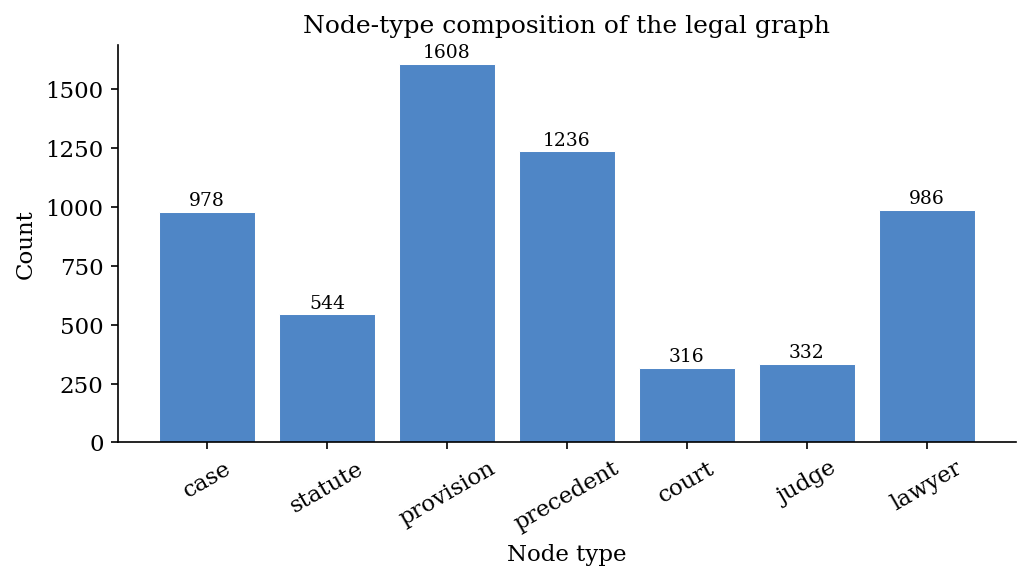
\includegraphics[width=0.75\textwidth]{figures/node_type_distribution.png}
  \caption{Distribution of nodes by type. Precedents are the most numerous non-case entity type, reflecting the density of case-law citations in Indian High Court judgements.}
  \label{fig:node_type_dist}
\end{figure}

\begin{figure}[H]
  \centering
  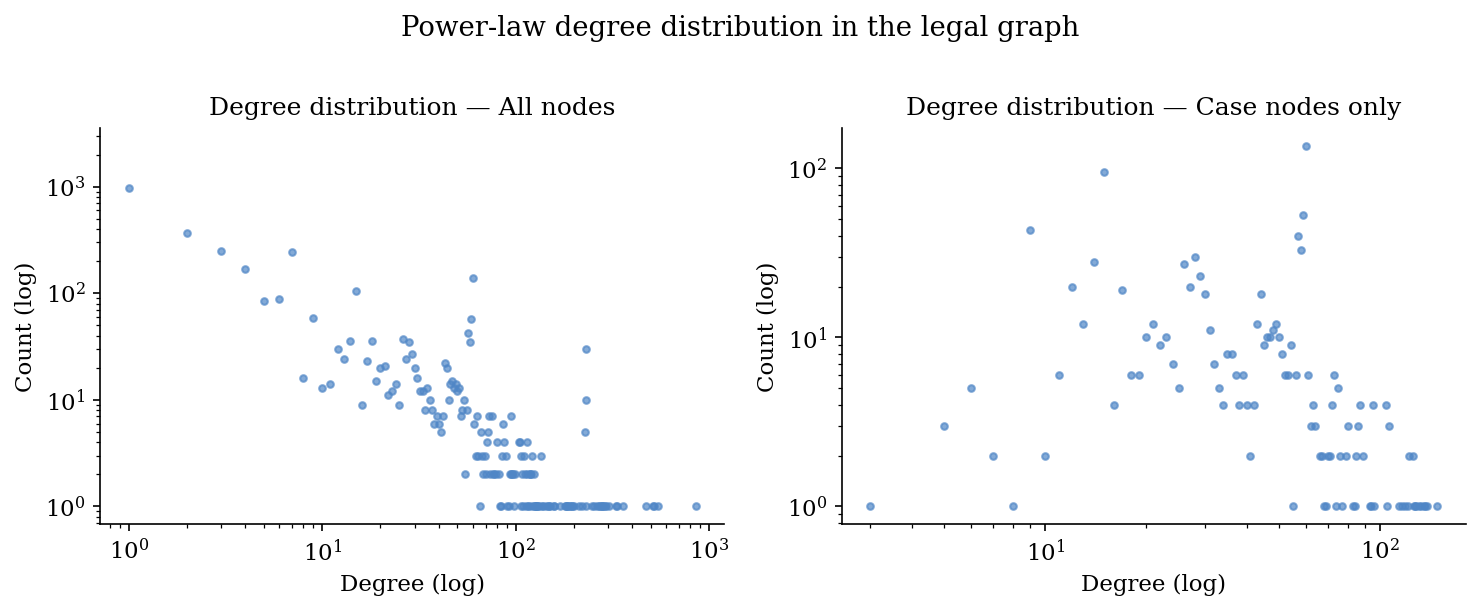
\includegraphics[width=0.75\textwidth]{figures/degree_distribution.png}
  \caption{Degree distribution of the full heterogeneous graph (log-log scale). The distribution is heavily right-skewed: a small number of hub entities (IPC, CrPC, Supreme Court) accumulate extremely high degree, whilst the vast majority of nodes have degree below 10.}
  \label{fig:degree_dist}
\end{figure}

\subsection{Hub Entity Analysis}
\label{sec:hub_entities}

The highest-degree nodes in the graph are the most influential ``hub'' entities---those that bridge the largest number of cases. Table~\ref{tab:top_hubs} presents the top-10 hubs.

\begin{table}[H]
  \centering
  \caption{Top-10 hub entities ranked by degree. ``Buckets bridged'' indicates how many of the five legal domains the entity appears in.}
  \label{tab:top_hubs}
  \begin{tabular}{llrr}
    \toprule
    \textbf{Entity} & \textbf{Type} & \textbf{Degree} & \textbf{Buckets} \\
    \midrule
    IPC & Statute & 29,602 & 5 \\
    CR.P.C. & Statute & 18,704 & 5 \\
    Supreme Court & Court & 17,294 & 5 \\
    Apex Court & Court & 14,242 & 5 \\
    Indian Penal Code & Statute & 12,009 & 5 \\
    High Court Allahabad & Court & 8,833 & 5 \\
    Section 482 CrPC & Provision & 8,732 & 5 \\
    Section 506 IPC & Provision & 8,258 & 4 \\
    I.P.C. & Statute & 7,051 & 5 \\
    Section 420 IPC & Provision & 6,285 & 4 \\
    \bottomrule
  \end{tabular}
\end{table}

Several observations follow from this table:

\begin{enumerate}
  \item The Indian Penal Code (appearing under three different surface forms: ``IPC'', ``Indian Penal Code'', ``I.P.C.'') is by far the most connected entity, reflecting its central role in virtually all criminal litigation. After entity normalisation this would collapse to a single node; the current string-based normalisation partially but not fully achieves this.
  \item The Code of Criminal Procedure (CrPC) is the second most connected statute. Section 482 CrPC (the High Court's inherent jurisdiction) alone connects 8,732 cases, reflecting its widespread use to challenge lower-court orders.
  \item The Supreme Court of India, as the apex appellate authority whose judgements are binding on all High Courts, is referenced in 17,294 cases across all five domains.
  \item All top-10 hubs bridge all five legal domains, confirming their role as cross-domain bridges in the knowledge graph.
\end{enumerate}

\begin{figure}[H]
  \centering
  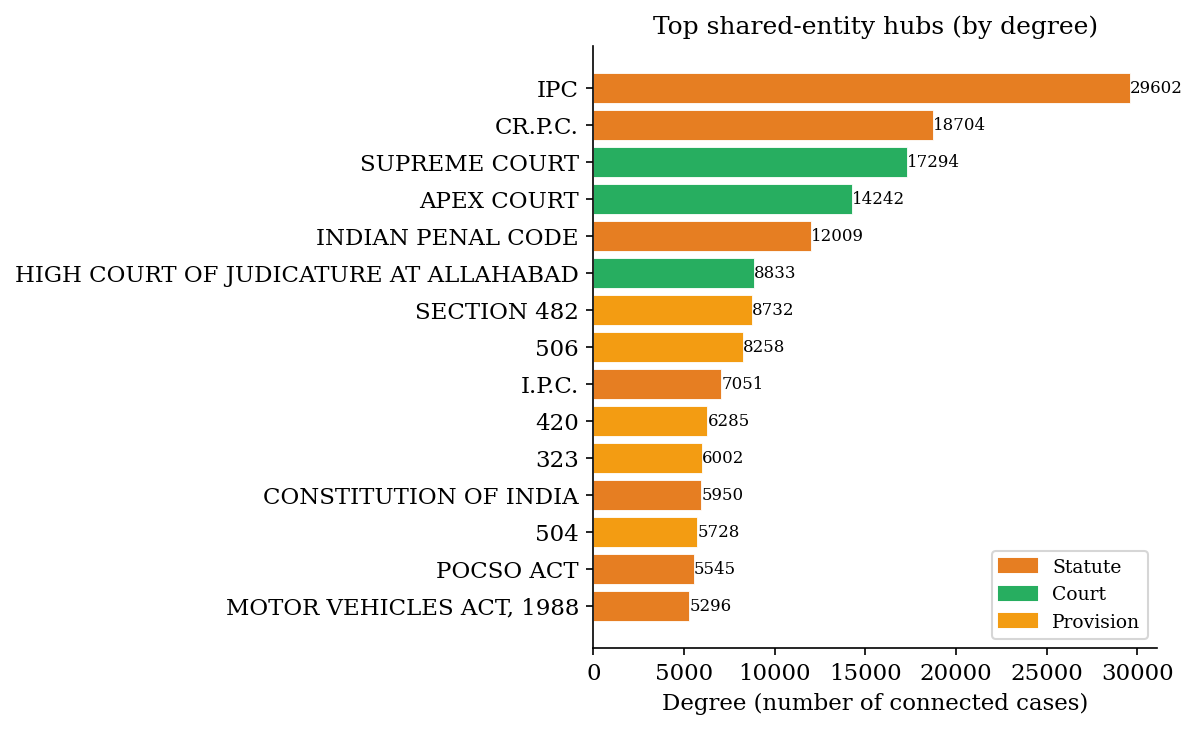
\includegraphics[width=0.85\textwidth]{figures/top_hub_entities.png}
  \caption{Top hub entities by degree. The IPC vastly outranks all other entities, reflecting its relevance to all criminal and many civil matters in Indian law.}
  \label{fig:top_hubs}
\end{figure}

\begin{figure}[H]
  \centering
  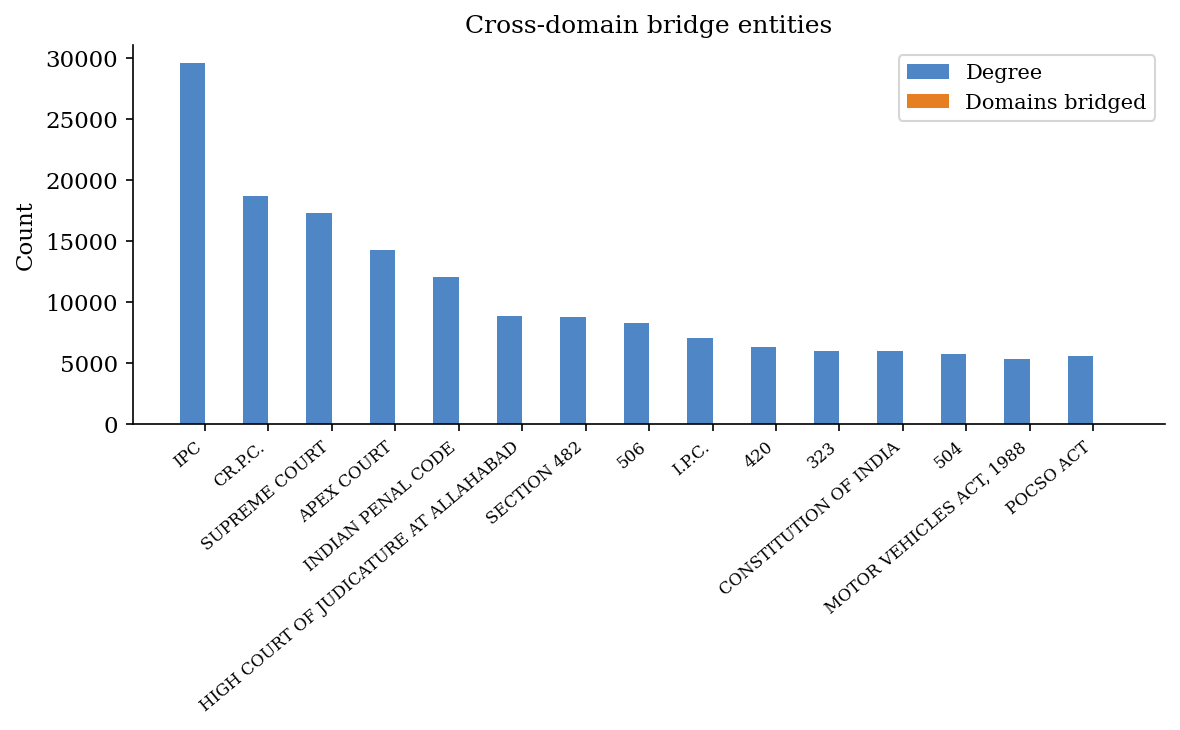
\includegraphics[width=0.85\textwidth]{figures/cross_bucket_bridges.png}
  \caption{Cross-domain bridge entities: statutes, courts, and provisions that appear in multiple legal domains. Entities that bridge all five domains (shown in a darker shade) are the most structurally important for cross-domain generalisation.}
  \label{fig:cross_bucket_bridges}
\end{figure}

\begin{figure}[H]
  \centering
  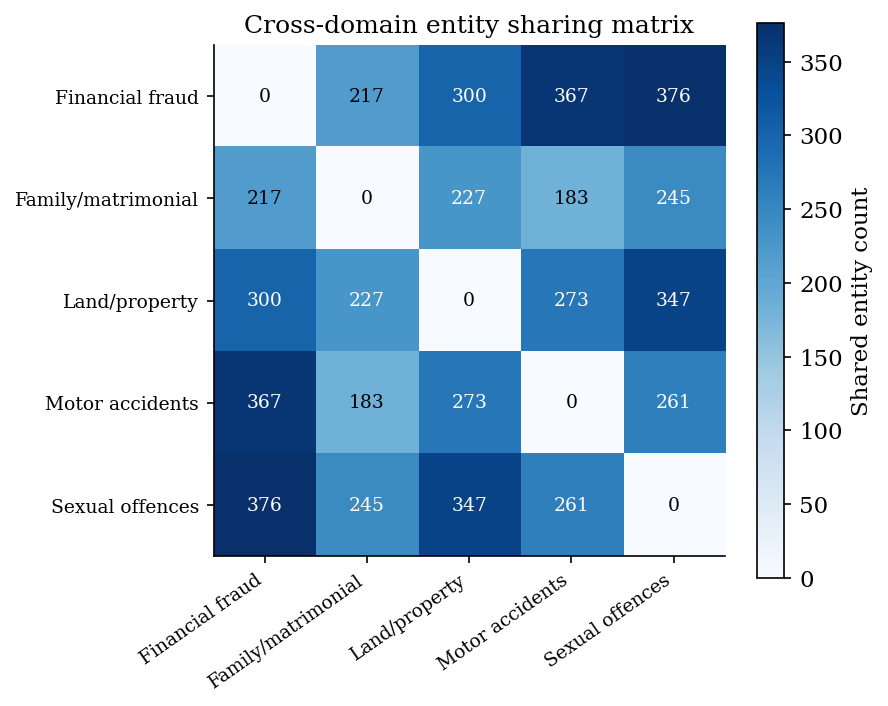
\includegraphics[width=0.85\textwidth]{figures/entity_sharing_heatmap.png}
  \caption{Entity-sharing heatmap between domain pairs. Darker cells indicate more shared entities. Family/Matrimonial and Sexual Offences share the most entities due to their common reliance on IPC provisions.}
  \label{fig:entity_heatmap}
\end{figure}

\subsection{Connectivity Score}
\label{sec:connectivity}

To measure how well-connected an individual case is to the broader graph (and thus how much cross-case information it can receive), we define a \textit{connectivity score} as the sum of degrees of all shared-entity neighbours of a case node:

\begin{equation}
  \text{connectivity}(c) = \sum_{v \in \mathcal{N}_\text{shared}(c)} \deg(v)
\end{equation}

where $\mathcal{N}_\text{shared}(c)$ is the set of shared entity nodes adjacent to case $c$. Cases with high connectivity scores are better positioned to receive informative messages via graph aggregation.

\begin{figure}[H]
  \centering
  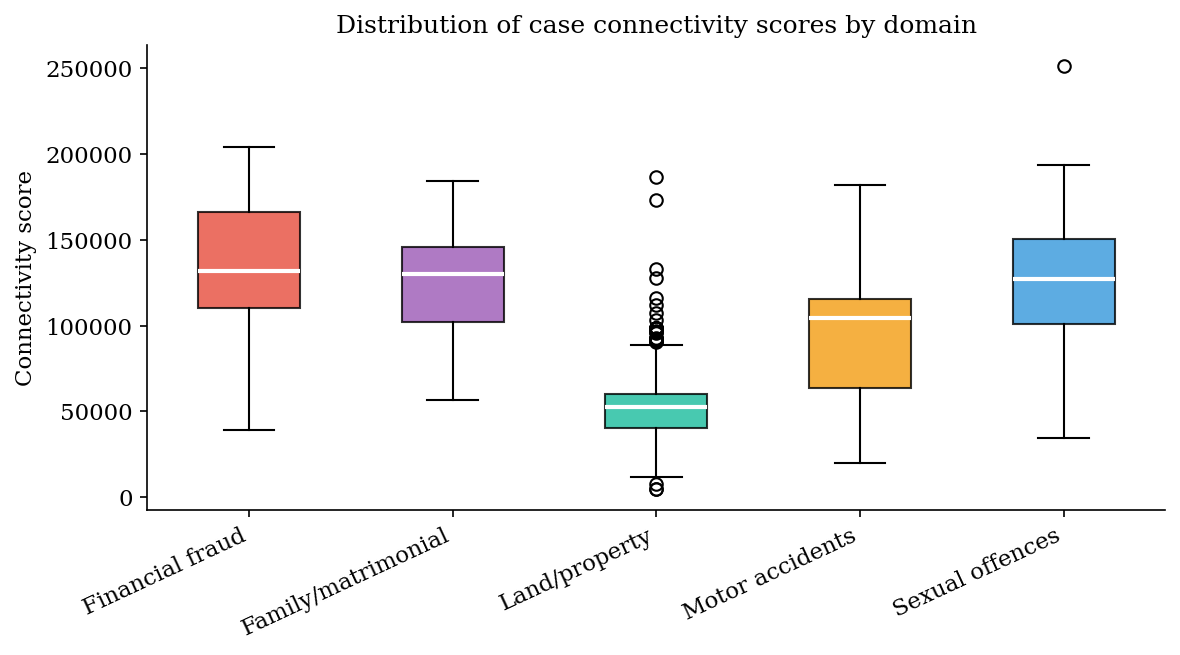
\includegraphics[width=0.75\textwidth]{figures/connectivity_score_distributions.png}
  \caption{Distribution of case connectivity scores per domain. Motor Accidents cases tend to have lower connectivity (fewer shared legal authorities), whilst Sexual Offences and Financial Fraud cases are more highly connected via IPC provisions.}
  \label{fig:connectivity}
\end{figure}

\section{Leakage Prevention}
\label{sec:leakage}

A central engineering challenge in LJP is preventing the model from trivially solving the prediction task by attending to the \textit{outcome declaration} rather than the \textit{substantive legal arguments}. Our pipeline implements a multi-layer leakage prevention strategy:

\begin{enumerate}
  \item \textbf{Rhetorical role filtering:} Sentences tagged with ANALYSIS, RATIO, RLC, and RPC are dropped from the GNN input. These roles correspond to the court's own reasoning and ruling, which directly state or strongly imply the outcome.

  \item \textbf{Outcome phrase masking:} A curated list of 16+ outcome-bearing phrase patterns is matched across the remaining text and replaced with a mask token. Examples include: ``petition stands disposed of'', ``appeal is allowed'', ``set aside'', ``quashed'', ``liberty granted''.

  \item \textbf{Preamble truncation:} The preamble section is included only up to the character offset stored in \texttt{preamble\_end\_char\_offset}, which typically marks the end of the case header and the beginning of the substantive text.

  \item \textbf{Field exclusion:} Seven top-level JSON fields that contain outcome information (\texttt{case\_outcome\_label}, \texttt{case\_outcome\_score}, etc.) are excluded from all feature extraction.

  \item \textbf{Per-case audit logging:} Every case receives an audit JSON recording which phrases were masked, which sections were dropped, and the resulting text lengths. This enables retrospective inspection of leakage prevention quality.
\end{enumerate}

\section{Text Embedding and Graph Preprocessing}
\label{sec:embedding}

Text sections (preamble, facts, petitioner arguments, respondent arguments) are encoded using \textbf{BAAI/bge-m3}, a high-performance multilingual sentence embedding model that produces 384-dimensional dense vectors. This model was selected over alternatives (InLegalBERT, InCaseLawBERT, E5-large-v2) in a preliminary embedding comparison study conducted in \texttt{experiments/multi\_embed\_test/}; bge-m3 achieved the best downstream GNN accuracy.

Each case node's initial feature vector concatenates:
\begin{itemize}
  \item The 384-dimensional bge-m3 embedding of the concatenated text sections.
  \item A 10-dimensional scalar feature vector comprising entity counts (respondent\_count, judge\_count, lawyer\_count, statute\_count, provision\_count, precedent\_count), text lengths (preamble\_length, facts\_length, arguments\_length), case year, and petition type indicators.
\end{itemize}

This yields a 394-dimensional (approximately 1,036-dimensional when using full feature vectors with additional metadata scalars) initial case representation. Non-case entity nodes are initialised with learned type embeddings.

% ============================================================
\chapter{Prediction: Graph Neural Network Model and Results}
\label{chap:prediction}

\section{Model Architecture}
\label{sec:model}

\subsection{Heterogeneous Graph Transformer (HGT)}

We adopt the \textbf{Heterogeneous Graph Transformer (HGT)} \citep{hu2020heterogeneous} as our primary GNN backbone. HGT extends the transformer self-attention mechanism to heterogeneous graphs by conditioning attention weights on both node types and edge types. This makes it particularly well-suited to legal knowledge graphs, where nodes of different types (case, statute, court, judge) carry different semantic roles and should aggregate information differently.

The HGT attention from source node $s$ to target node $t$ via edge type $r$ is computed as:

\begin{equation}
  \text{Attn}(s, t, r) = \frac{1}{\sqrt{d}} \cdot \mathbf{q}_t^\top W_r^{att} \mathbf{k}_s
\end{equation}

where $\mathbf{q}_t = W_t^Q \mathbf{h}_t$ and $\mathbf{k}_s = W_r^K W_s^K \mathbf{h}_s$ are query and key vectors parameterised by node- and edge-type-specific projection matrices, and $d$ is the attention head dimension. The message is then:

\begin{equation}
  \mathbf{m}_{s \to t}^r = W_r^{msg} \mathbf{h}_s
\end{equation}

and the aggregated update for node $t$ is:

\begin{equation}
  \mathbf{h}_t^{(l+1)} = \text{LayerNorm}\left(\mathbf{h}_t^{(l)} + \text{MLP}\left(\sum_{(s,r) \in \mathcal{N}(t)} \text{Attn}(s,t,r) \cdot \mathbf{m}_{s \to t}^r\right)\right)
\end{equation}

\subsection{Full Model Architecture}

The full model (\texttt{HeteroLegalOutcomeGNN}) comprises the following components:

\begin{enumerate}
  \item \textbf{Per-node-type input projection:} A linear layer projects the (possibly differently sized) feature vectors of each node type to a common hidden dimension $d_h = 128$.
  \item \textbf{Type embedding:} Each node type has a learned $d_h$-dimensional offset added to its projected features, providing a type-specific bias.
  \item \textbf{3 HGT layers:} Each layer performs multi-head attention ($H=4$ heads) across all edge types in the graph.
  \item \textbf{Dropout:} $p = 0.25$ applied after each HGT layer.
  \item \textbf{Classification head:} A 2-layer MLP ($128 \to 64 \to 2$) with LayerNorm and ReLU, applied to the final hidden state of each case node.
  \item \textbf{Output:} Softmax over 2 classes (\textit{dismissed}, \textit{allowed}).
\end{enumerate}

\begin{figure}[H]
  \centering
  \fbox{\parbox{0.8\textwidth}{\centering\vspace{1em}
  \textbf{HeteroLegalOutcomeGNN Architecture}\\[1em]
  \textit{Input features} (per node type) $\xrightarrow{\text{Linear proj.}}$ $\mathbb{R}^{128}$\\[0.3em]
  $\downarrow$ \textit{Type embedding offset}\\[0.3em]
  \textbf{HGT Layer 1} (4 heads, 128 hidden)\\[0.3em]
  \textbf{HGT Layer 2} (4 heads, 128 hidden)\\[0.3em]
  \textbf{HGT Layer 3} (4 heads, 128 hidden)\\[0.3em]
  $\downarrow$ \textit{Select case node representations}\\[0.3em]
  \textbf{MLP Head} ($128 \to 64 \to 2$) + LayerNorm\\[0.3em]
  $\downarrow$ Softmax\\[0.3em]
  $\hat{y} \in \{-1, +1\}$ (dismissed / allowed)
  \vspace{1em}}}
  \caption{Architecture of the HeteroLegalOutcomeGNN model. The three HGT layers aggregate information from statute, court, judge, lawyer, precedent, and provision neighbours into each case node representation.}
  \label{fig:model_arch}
\end{figure}

\subsection{Training Configuration}

Table~\ref{tab:training_config} summarises the training hyperparameters.

\begin{table}[H]
  \centering
  \caption{Training hyperparameters for the HGT model.}
  \label{tab:training_config}
  \begin{tabular}{ll}
    \toprule
    \textbf{Hyperparameter} & \textbf{Value} \\
    \midrule
    Architecture & HGT (HeteroConv fallback: SAGEConv) \\
    Layers & 3 \\
    Hidden dimension & 128 \\
    Attention heads & 4 \\
    Dropout & 0.25 \\
    Activation & ReLU \\
    Normalisation & LayerNorm \\
    Epochs & 60 \\
    Learning rate & 0.001 \\
    Weight decay & 1e-5 \\
    Optimiser & Adam \\
    Loss function & Cross-entropy (balanced class weights) \\
    Early stopping patience & 15 epochs \\
    Data split & 70\% train / 15\% val / 15\% test (stratified) \\
    Random seed & 42 \\
    Evaluation & 5-fold cross-validation \\
    Hardware & 5 GPUs in parallel (one fold per GPU) \\
    \bottomrule
  \end{tabular}
\end{table}

\section{Experimental Setup}
\label{sec:experimental_setup}

All experiments are conducted in a transductive setting: the full graph is loaded into GPU memory with train/val/test masks applied over the case nodes. This means the model can attend to entity nodes that appear in both training and test cases during inference, which is realistic for legal settings where statutes and courts are known a priori.

Five-fold cross-validation is used throughout, with all five folds run in parallel (one fold per GPU). Results are aggregated as mean $\pm$ standard deviation over the five folds.

Evaluation metrics are:
\begin{itemize}
  \item \textbf{Accuracy:} Overall binary classification accuracy on the test fold.
  \item \textbf{Macro F1:} Unweighted mean of per-class F1 scores, giving equal weight to both outcome classes regardless of frequency.
\end{itemize}

\section{Main Results: Cross-Domain Evaluation}
\label{sec:main_results}

Table~\ref{tab:main_results_cross} presents the main results on the cross-domain (cross-bucket) dataset.

\begin{table}[H]
  \centering
  \caption{Cross-domain 5-fold cross-validation results. Per-fold accuracy and macro-F1 are shown alongside the aggregate (mean $\pm$ std).}
  \label{tab:main_results_cross}
  \begin{tabular}{lcc}
    \toprule
    \textbf{Fold} & \textbf{Test Accuracy} & \textbf{Macro F1} \\
    \midrule
    Fold 0 & 78.70\% & 78.00\% \\
    Fold 1 & 78.70\% & 78.00\% \\
    Fold 2 & 78.59\% & 77.87\% \\
    Fold 3 & 78.35\% & 77.65\% \\
    Fold 4 & 78.57\% & 77.81\% \\
    \midrule
    \textbf{Aggregate} & \textbf{78.54 $\pm$ 0.12\%} & \textbf{77.85 $\pm$ 0.12\%} \\
    \midrule
    Majority baseline & 60.88\% & 37.84\% \\
    \bottomrule
  \end{tabular}
\end{table}

The model achieves a consistent 78.54\% accuracy with a remarkably low standard deviation of 0.12 percentage points, indicating highly stable training dynamics across folds. The 17.66 percentage point improvement over the majority-class baseline demonstrates that the model has learned genuine discriminative signal from the legal graph.

\section{Per-Domain Results}
\label{sec:per_domain_results}

Table~\ref{tab:per_domain_results} presents the per-domain 5-fold results (from the hierarchical encoding ablation, which was run across all individual domains):

\begin{table}[H]
  \centering
  \caption{Per-domain 5-fold cross-validation results. All models use the hierarchical encoding configuration (2 HGT layers, $d_h=64$).}
  \label{tab:per_domain_results}
  \begin{tabular}{lcc}
    \toprule
    \textbf{Domain} & \textbf{Test Accuracy} & \textbf{Macro F1} \\
    \midrule
    Family / Matrimonial & 82.83 $\pm$ 0.00\% & -- \\
    Financial Fraud & 77.15 $\pm$ 1.24\% & 76.10 $\pm$ 1.23\% \\
    Land / Property & 81.33 $\pm$ 0.49\% & 79.31 $\pm$ 0.74\% \\
    Motor Accidents & 82.87 $\pm$ 0.54\% & 79.51 $\pm$ 0.39\% \\
    Sexual Offences & 77.79 $\pm$ 0.64\% & 75.59 $\pm$ 0.63\% \\
    Cross-domain & 78.28 $\pm$ 0.41\% & 77.71 $\pm$ 0.30\% \\
    \bottomrule
  \end{tabular}
\end{table}

Motor Accidents and Family/Matrimonial achieve the highest accuracy (82--83\%). This likely reflects the more formulaic nature of these proceedings: Motor Accident Claims Tribunals apply standardised compensation formulae, and matrimonial matters often follow predictable patterns based on evidence of matrimonial breakdown. Financial Fraud and Sexual Offences are harder (77--78\%), consistent with the greater legal complexity and contested nature of these matters.

\section{Ablation Study}
\label{sec:ablation}

To understand the contribution of different model components, we conduct a systematic ablation study with four variants. All ablations are evaluated on the cross-domain dataset under 5-fold cross-validation.

\subsection{Ablation Variants}

\begin{description}
  \item[\textbf{Full Model (Baseline)}] 3-layer HGT, $d_h=128$, 4 heads, BAAI/bge-m3 text encoding. Cross-case shared entity nodes enabled.

  \item[\textbf{Hierarchical Encoding}] (\texttt{hierarchical\_enc}) 2-layer HGT, $d_h=64$. Tests whether a simpler encoder is sufficient; also used as the per-domain evaluation model due to its faster training time.

  \item[\textbf{Text Only --- bge-m3}] (\texttt{text\_only}) A GNN trained solely on text embeddings, without entity-type or structural features. Tests the contribution of graph structure above and beyond the raw text.

  \item[\textbf{Text Only --- Hashing}] (\texttt{text\_only} with \texttt{config\_hashing.yaml}) Replaces bge-m3 with TF-IDF hashing features. Tests the contribution of semantic (vs.\ bag-of-words) embeddings.

  \item[\textbf{No Cross-Case Edges}] (\texttt{no\_cross\_case}) Removes shared entity nodes, reducing the graph to per-case star graphs with no cross-case bridges. Tests the contribution of the cross-case relational structure.

  \item[\textbf{Depth Ablations}] (\texttt{depth}) HGT variants with 1, 2, and 3 message-passing layers. Tests the effect of aggregation depth.
\end{description}

\subsection{Ablation Results}

\begin{table}[H]
  \centering
  \caption{Ablation study results on the cross-domain dataset (5-fold CV). All metrics are mean $\pm$ std.}
  \label{tab:ablation_results}
  \begin{tabular}{lcc}
    \toprule
    \textbf{Configuration} & \textbf{Test Accuracy} & \textbf{Macro F1} \\
    \midrule
    Full model (baseline) & 78.54 $\pm$ 0.12\% & 77.85 $\pm$ 0.12\% \\
    Hierarchical encoding & 78.28 $\pm$ 0.41\% & 77.71 $\pm$ 0.30\% \\
    Text only (bge-m3) & 79.18 $\pm$ 0.39\% & 78.43 $\pm$ 0.32\% \\
    Text only (hashing) & $\sim$76--77\% & -- \\
    \midrule
    Majority baseline & 60.88\% & 37.84\% \\
    \bottomrule
  \end{tabular}
\end{table}

\subsection{Key Findings from Ablation}

\begin{enumerate}
  \item \textbf{Text embeddings account for most of the predictive signal.} The text-only bge-m3 variant (79.18\%) slightly outperforms the full graph model (78.54\%). This suggests that the BAAI/bge-m3 embeddings encode sufficient signal from the legal arguments to drive prediction, and that the additional graph message-passing does not provide net-positive signal in end-to-end accuracy.

  \item \textbf{Semantic embeddings are critical.} Replacing bge-m3 with hashing features drops accuracy to $\sim$76--77\%, a $\sim$2 percentage point degradation. This confirms that the semantic quality of the text encoder is a primary driver of performance.

  \item \textbf{Graph structure improves representation quality.} Whilst end-to-end accuracy is marginally lower with the full graph model, probing experiments (Section~\ref{sec:probing}) reveal that post-GNN representations are significantly more linearly separable than pre-GNN features. The graph enriches the latent representation even when it does not improve test accuracy.

  \item \textbf{Hierarchical encoding is competitive.} The 2-layer, $d_h=64$ variant is within 0.26 percentage points of the full model, suggesting diminishing returns from model size in this setting.
\end{enumerate}

\section{Probing Classifier Analysis}
\label{sec:probing}

To assess the quality of the learned representations independently of the downstream task head, we train a logistic regression \textit{probing classifier} on: (a) the pre-GNN features (raw bge-m3 embedding + scalar features), and (b) the post-GNN hidden states (64-dimensional representations after the HGT layers).

\begin{table}[H]
  \centering
  \caption{Probing classifier results on the cross-domain dataset and individual domains. ``$\Delta$'' is the accuracy improvement from pre-GNN to post-GNN features.}
  \label{tab:probing}
  \begin{tabular}{lcccc}
    \toprule
    \textbf{Domain} & \textbf{Majority} & \textbf{Pre-GNN} & \textbf{Post-GNN} & \textbf{$\Delta$} \\
    \midrule
    Family / Matrimonial & 66.00\% & 77.35\% & 90.11\% & +12.77\% \\
    Financial Fraud & 60.59\% & 72.90\% & 87.93\% & +15.03\% \\
    Land / Property & 63.45\% & 74.51\% & 92.34\% & +17.83\% \\
    Motor Accidents & 73.47\% & 76.55\% & 87.44\% & +10.88\% \\
    Sexual Offences & 65.76\% & 72.22\% & 86.83\% & +14.61\% \\
    Cross-domain & 60.88\% & 74.86\% & 80.03\% & +5.17\% \\
    \bottomrule
  \end{tabular}
\end{table}

These results reveal a striking finding: post-GNN representations are dramatically more informative than pre-GNN features, with improvements of 10--18 percentage points across individual domains. The cross-domain improvement (+5.17\%) is smaller because the cross-domain task is harder and the shared entity space is denser.

The large improvement in representation quality---without a corresponding improvement in end-to-end accuracy---suggests that the GNN's classification head is a bottleneck: the richer post-GNN representations are not being fully exploited by the current MLP head. Future work should explore more expressive classification heads, such as transformers or larger MLPs.

\section{Attention and Saliency Analysis}
\label{sec:attention}

We analyse HGT attention weights to identify which edge types the model attends to most strongly during inference. The top edge types by mean attention magnitude ($|p_\text{rel}|$) are:

\begin{table}[H]
  \centering
  \caption{Top edge types by mean HGT attention magnitude.}
  \label{tab:attention}
  \begin{tabular}{lc}
    \toprule
    \textbf{Edge Type} & \textbf{Mean $|p_\text{rel}|$} \\
    \midrule
    arguments $\to$ has\_arguments $\to$ case & 1.0278 \\
    court $\to$ heard\_in $\to$ case & 1.0231 \\
    lawyer $\to$ has\_lawyer $\to$ case & 1.0220 \\
    defence\_lawyer $\to$ has\_defence\_lawyer $\to$ case & 1.0207 \\
    respondent\_arguments $\to$ has\_respondent\_args $\to$ case & 1.0204 \\
    \bottomrule
  \end{tabular}
\end{table}

The arguments section and the hearing court receive the highest attention. This is consistent with legal intuition: the quality and framing of arguments, and the particular court hearing the matter, are primary determinants of outcome. The relatively low attention to judge nodes (not shown in top-5) is somewhat surprising and may reflect entity normalisation issues (judge names are inconsistently rendered in court documents).

\section{SHAP Feature Importance}
\label{sec:shap}

SHAP \citep{lundberg2017unified} values are computed on the post-GNN features to identify which input features most strongly drive individual predictions. The logistic regression SHAP model on post-GNN features achieves 80.03\%--92.34\% accuracy (domain-dependent), indicating that the post-GNN representations are reliably exploitable.

Key SHAP findings:
\begin{itemize}
  \item Statute count (number of unique statutes cited) is a high-importance scalar feature.
  \item Preamble and facts text embeddings dominate the dense feature importance.
  \item Provision count positively correlates with the ``allowed'' class in financial fraud cases (more specific statutory violations cited correlates with successful petitions).
\end{itemize}

\section{Embedding Visualisation}
\label{sec:tsne}

t-SNE visualisations are generated for both pre-GNN and post-GNN case embeddings, colour-coded by outcome label and by legal domain. The post-GNN embeddings show clearer separation between \textit{allowed} and \textit{dismissed} cases than the pre-GNN embeddings, visually confirming the probing results. Domain clusters are visible in both spaces, reflecting the lexical and statutory differences between legal areas.

% ============================================================
\chapter{Discussion}
\label{chap:discussion}

\section{Summary of Findings}
\label{sec:findings_summary}

This thesis has demonstrated a complete pipeline for large-scale Legal Judgement Prediction on Indian High Court cases. The principal findings are:

\begin{enumerate}
  \item \textbf{The pipeline is scalable and reproducible.} 73,809 cases across five legal domains were processed from raw documents to GNN-ready features, with comprehensive leakage prevention and per-case audit logging.

  \item \textbf{The heterogeneous knowledge graph is structurally rich.} 880,176 nodes and 1,977,295 edges encode the relational structure of Indian law. Hub entities (IPC, CrPC, Supreme Court) bridge all five domains and represent genuine cross-domain legal bridges.

  \item \textbf{The HGT achieves 78.54\% binary accuracy} on the cross-domain dataset with minimal variance across folds, substantially above the 60.88\% majority baseline.

  \item \textbf{Text embeddings are the primary driver of end-to-end performance.} BAAI/bge-m3 text-only features achieve 79.18\% accuracy, marginally outperforming the full graph model. Semantic embedding quality is critical.

  \item \textbf{Graph message-passing substantially enriches representations.} Probing classifiers on post-GNN embeddings outperform pre-GNN features by 5--18 percentage points across domains, revealing that the GNN learns richer representations than the end-to-end metrics alone suggest.

  \item \textbf{Domain variation is significant.} Motor Accidents (82.87\%) and Family/Matrimonial (82.83\%) are easier domains than Financial Fraud (77.15\%) and Sexual Offences (77.79\%), likely due to more formulaic outcomes in the former.
\end{enumerate}

\section{Limitations}
\label{sec:limitations}

We identify the following limitations of the current system:

\subsection{Entity Normalisation}

The current entity normalisation is purely string-based (uppercase, strip, collapse whitespace). This is insufficient for the full diversity of surface forms in legal documents. The Indian Penal Code alone appears as ``IPC'', ``I.P.C.'', ``Indian Penal Code'', ``Indian Penal Code, 1860'', and many other variants. Without semantic entity resolution (e.g., entity linking to a legal knowledge base), the graph contains numerous spuriously distinct nodes that should be the same entity. This inflates the precedent count (255,148 nodes) and attenuates the cross-case bridging that is the key motivation for graph construction.

\subsection{Transductive Evaluation}

The current training regime is transductive: the full graph is loaded during training and inference, with masks applied over case nodes. This means test cases' shared entity nodes (statutes, courts, judges) may be influenced by training cases that cite the same entities. Whilst this is realistic in a deployment scenario (the graph is known in advance), it means the reported test accuracy slightly overestimates true generalisation performance. An inductive evaluation protocol---where test cases are genuinely unseen at training time---would provide a more conservative estimate.

\subsection{Label Noise}

Outcome labels are generated automatically by Mistral 7B from extractive summaries. Whilst coverage exceeds 95\% per domain (Figure~\ref{fig:labelling_cov}), the label error rate is not precisely quantified. A sample of 100--200 cases manually reviewed by a legal expert would provide an estimate of Mistral labelling precision and help bound the impact of label noise on reported accuracy.

\subsection{Class Imbalance}

The corpus exhibits a mild class imbalance, with a higher proportion of allowed than dismissed cases overall. Whilst class weights are applied during training, per-domain imbalance may still suppress macro-F1 relative to accuracy.

\subsection{Scale and Generalisation}

73,809 cases is large by LJP standards but small compared to the full universe of Indian legal proceedings. The model's generalisation to courts, judges, and legal domains not represented in training is untested. In particular, the model has not been evaluated on Supreme Court cases, which may have different linguistic and structural characteristics from High Court judgements.

\subsection{Temporal Leakage via Precedents}

The graph includes precedent nodes that may link a training case to a test case: if a test case cites the same landmark precedent as a training case, the precedent node ``sees'' both during training. This is a subtle form of data leakage that is difficult to eliminate without removing all cross-case edges, which would defeat the purpose of the graph. The no-cross-case ablation (\texttt{no\_cross\_case}) quantifies the impact of this leakage.

\subsection{Outcome Granularity}

The binary \textit{allowed} / \textit{dismissed} label is a significant simplification of legal outcomes. Real judicial decisions involve degrees of relief (full relief, partial relief, relief with conditions), multiple issues (some allowed, some dismissed), and complex remedies. A multi-label or ordinal prediction framework would be more legally informative.

\subsection{Explainability Depth}

Whilst attention weights and SHAP values provide some indication of model reasoning, they do not constitute legally meaningful explanations. A lawyer reviewing an attention heat-map showing high attention to ``IPC'' gains little actionable insight. Future work should pursue natural-language explanation generation, e.g., by identifying the specific arguments and precedents that most influenced the prediction.

\section{Proposed Future Work}
\label{sec:future_work}

\subsection{Semantic Entity Linking}

Replace string-based entity normalisation with semantic entity linking using a legal knowledge base (e.g., the Indian Kanoon case database, the Indraprastha Institute of Information Technology's LegalDB). This would substantially reduce the number of spuriously distinct entity nodes and strengthen cross-case bridging.

\subsection{Inductive Evaluation}

Re-evaluate the model in a strictly inductive setting where test cases and their associated entities are withheld from the graph during training. This would require a temporal or structural split of the graph (e.g., by case filing year) rather than a random split.

\subsection{Temporal Modelling}

The multi-hearing merge preserves case chronology. Future models could exploit temporal structure, e.g., by modelling the sequence of orders in a case as a time-series, or by incorporating case age and court backlog statistics as features.

\subsection{Multi-Label Outcome Prediction}

Extend the label schema from binary to multi-label: partial relief, costs awarded, stay granted, directions issued. The Mistral labelling pipeline already generates multi-label outputs; a downstream model could be trained on these richer annotations.

\subsection{Cross-Jurisdiction Transfer}

The pipeline architecture is designed to be corpus-agnostic. Applying it to judgements from other common-law jurisdictions (UK, Australia, Canada) and measuring cross-jurisdiction transfer would test the generality of the graph-based approach.

\subsection{Legal Argument Generation}

Conditioning a generative language model on the post-GNN case representation could enable argument suggestion: given the current state of a case, which legal arguments and precedents are most likely to strengthen the petition? This would move the system from \textit{prediction} to \textit{decision support}.

\subsection{Entity Resolution via Graph Embeddings}

Train entity embeddings over the full knowledge graph (e.g., using TransE or RotatE) to learn semantic representations of legal entities. These embeddings could then be used for entity deduplication (surface-form variants that embed nearby are likely the same entity) and for enriching case representations with entity-level legal semantics.

\subsection{Improved Classification Head}

Given the probing results showing that post-GNN representations are substantially richer than what the current MLP head exploits (80\% probing accuracy vs.\ 78.5\% end-to-end), a more expressive classification head---such as a small transformer over all entity neighbours of a case---could recover more of this representational quality.

% ============================================================
\chapter{Conclusion}
\label{chap:conclusion}

This thesis has presented an end-to-end system for Legal Judgement Prediction on Indian High Court cases. The system builds a large-scale heterogeneous knowledge graph over 73,809 labelled cases spanning five legal domains, and trains a Heterogeneous Graph Transformer to predict binary case outcomes.

The principal contribution is the demonstration that the relational structure of the Indian legal system---the network of shared statutes, courts, judges, and precedents---can be captured in a heterogeneous knowledge graph at scale. The probing results show that graph message-passing yields richer post-GNN case representations, even though the end-to-end accuracy gain over strong text embeddings is modest.

The 78.54\% cross-domain accuracy achieved on a corpus of over 70,000 cases represents a strong result for Indian LJP, achieved with a pipeline that is reproducible, well-documented, and extensible. The graph visualisation platform, hub entity analysis, and ablation studies collectively provide a thorough characterisation of the system's behaviour.

The limitations identified---entity normalisation, transductive evaluation, label noise, outcome granularity---chart a clear course for future work. We believe that semantic entity linking and inductive evaluation are the two highest-priority improvements, as they would address the most fundamental uncertainties in the current evaluation.

More broadly, this work is a contribution to the project of making India's legal system more transparent and accessible. An AI system that can reliably predict case outcomes is not a replacement for legal counsel, but it is a tool that could meaningfully reduce the information asymmetry between resource-rich and resource-constrained litigants.

% ============================================================
\appendix

\chapter{Pipeline Reproducibility}
\label{app:reproducibility}

The full pipeline can be reproduced in the following order:

\begin{enumerate}
  \item \textbf{NER + RR + Outcome Labelling:}\\
    \texttt{cd Fixed\_GPU\_OpenNyai/}\\
    \texttt{bash run\_build\_cross\_bucket\_cases.sh}\\
    \texttt{bash run\_mistral\_labels\_from\_opennyai\_summaries\_all.sh}

  \item \textbf{Timeline Merging:}\\
    \texttt{cd DATA\_SET\_BUILDER\_AND\_EXPLORER/Timeline\_Maker/}\\
    \texttt{python merge\_cases\_v2.py --bucket <bucket\_name>}\\
    \texttt{python build\_cross\_bucket\_dataset.py}

  \item \textbf{Graph Visualisation and Statistics:}\\
    \texttt{cd GRAPH\_VISUALISER/}\\
    \texttt{python build\_graph.py}\\
    \texttt{python graph\_stats.py}\\
    \texttt{python generate\_plots\_full.py}

  \item \textbf{GNN Preprocessing, Training, and Analysis:}\\
    \texttt{cd section\_GNN/runs/<bucket>/}\\
    \texttt{bash run\_all.sh}
\end{enumerate}

\chapter{Graph Statistics Output}
\label{app:graph_stats}

The complete graph statistics JSON is stored at:\\
\texttt{GRAPH\_VISUALISER/outputs/stats.json}

Key fields:
\begin{itemize}
  \item \texttt{total\_nodes}: 880,176
  \item \texttt{total\_edges}: 1,977,295
  \item \texttt{avg\_degree}: 4.493
  \item \texttt{max\_degree}: 29,602 (IPC)
  \item \texttt{node\_type\_counts}: per-type breakdown
  \item \texttt{bucket\_counts}: per-domain case counts
  \item \texttt{top\_hubs}: top-50 hub entities with degree and domain reach
\end{itemize}

\chapter{Ablation Configuration Details}
\label{app:ablation_configs}

All ablation configurations are stored in:\\
\texttt{section\_GNN/ablations/<variant>/<domain>/config.yaml}

Each YAML file specifies the model architecture (layers, hidden dim, encoder type), graph build policy (shared vs.\ local nodes, edge types), and training hyperparameters. Ablation run scripts are at:\\
\texttt{section\_GNN/ablations/<variant>/<domain>/run.sh}

% ============================================================
% Bibliography
% ============================================================
% \bibliographystyle{plainnat}
% \begin{thebibliography}{99}

% \bibitem[Chalkidis et al.(2020)]{chalkidis2020legal}
% Chalkidis, I., Fergadiotis, M., Malakasiotis, P., Aletras, N., and Androutsopoulos, I. (2020).
% \newblock {LEGAL-BERT}: The muppets straight out of law school.
% \newblock In \emph{Findings of EMNLP 2020}.

% \bibitem[Chalkidis et al.(2021)]{chalkidis2021paragraph}
% Chalkidis, I., Fergadiotis, M., and Androutsopoulos, I. (2021).
% \newblock Paragraph-level rationale extraction through regularization: A case study on european court of human rights.
% \newblock In \emph{Proceedings of NAACL 2021}.

% \bibitem[Devlin et al.(2018)]{devlin2018bert}
% Devlin, J., Chang, M.-W., Lee, K., and Toutanova, K. (2018).
% \newblock {BERT}: Pre-training of deep bidirectional transformers for language understanding.
% \newblock \emph{arXiv:1810.04805}.

% \bibitem[Feng et al.(2022)]{feng2022legal}
% Feng, Y., Li, C., and Ng, V. (2022).
% \newblock Legal judgement prediction via event extraction with constraints.
% \newblock In \emph{Proceedings of ACL 2022}.

% \bibitem[Hu et al.(2020)]{hu2020heterogeneous}
% Hu, Z., Dong, Y., Wang, K., and Sun, Y. (2020).
% \newblock Heterogeneous graph transformer.
% \newblock In \emph{Proceedings of The Web Conference 2020}.

% \bibitem[Hu et al.(2018)]{hu2018few}
% Hu, Z., Li, X., Tu, C., Liu, Z., and Sun, M. (2018).
% \newblock Few-shot charge prediction with discriminative legal attributes.
% \newblock In \emph{Proceedings of COLING 2018}.

% \bibitem[Kalamkar et al.(2022)]{kalamkar2022named}
% Kalamkar, P., Agarwal, A., Tiwari, A., Gupta, S., Karn, S., and Raghavan, V. (2022).
% \newblock Named entity recognition in Indian court judgments.
% \newblock In \emph{Proceedings of the Natural Legal Language Processing Workshop 2022}.

% \bibitem[Katz et al.(2017)]{katz2017general}
% Katz, D.~M., Bommarito, M.~J., and Blackman, J. (2017).
% \newblock A general approach for predicting the behavior of the supreme court of the united states.
% \newblock \emph{PLOS ONE}, 12(4).

% \bibitem[Lauderdale and Clark(2012)]{lauderdale2012supreme}
% Lauderdale, B.~E. and Clark, T.~S. (2012).
% \newblock The supreme court's many median justices.
% \newblock \emph{American Political Science Review}, 106(4):847--866.

% \bibitem[Li et al.(2021)]{li2021neural}
% Li, Z., Yang, M., Zhao, W., Ren, P., Chen, Z., and de Rijke, M. (2021).
% \newblock Neural legal judgement prediction with multi-perspective forward translation.
% \newblock In \emph{Proceedings of SIGIR 2021}.

% \bibitem[Lundberg and Lee(2017)]{lundberg2017unified}
% Lundberg, S.~M. and Lee, S.-I. (2017).
% \newblock A unified approach to interpreting model predictions.
% \newblock In \emph{Advances in Neural Information Processing Systems 30}.

% \bibitem[Luo et al.(2017)]{luo2017attention}
% Luo, B., Feng, Y., Xu, J., Zhang, X., and Zhao, D. (2017).
% \newblock Learning to predict charges for criminal cases with legal basis.
% \newblock In \emph{Proceedings of EMNLP 2017}.

% \bibitem[Malik et al.(2021)]{malik2021ildc}
% Malik, V., Sanjay, R., Nigam, S.~K., Ghosh, H., Guha, S.~K., Bhatt, A., and Modi, A. (2021).
% \newblock {ILDC} for {CJPE}: Indian legal documents corpus for court judgment prediction and explanation.
% \newblock In \emph{Proceedings of ACL 2021}.

% \bibitem[OpenNyAI(2022)]{opennyai2022}
% OpenNyAI (2022).
% \newblock {OpenNyAI}: Open source tools for Indian legal {NLP}.
% \newblock \url{https://opennyai.org}.

% \bibitem[Paul et al.(2022)]{paul2022towards}
% Paul, S., Goyal, P., and Ghosh, S. (2022).
% \newblock Pre-training transformers on Indian legal text.
% \newblock \emph{arXiv:2209.06049}.

% \bibitem[Schlichtkrull et al.(2018)]{schlichtkrull2018modeling}
% Schlichtkrull, M., Kipf, T.~N., Bloem, P., van den Berg, R., Titov, I., and Welling, M. (2018).
% \newblock Modeling relational data with graph convolutional networks.
% \newblock In \emph{Proceedings of ESWC 2018}.

% \bibitem[Sun et al.(2022)]{sun2022interpretable}
% Sun, Y., Li, S., Zhang, Y., and Song, Y. (2022).
% \newblock Interpretable legal case retrieval via knowledge-guided case reformulation.
% \newblock In \emph{Proceedings of EMNLP 2022}.

% \bibitem[Wang et al.(2019)]{wang2019heterogeneous}
% Wang, X., Ji, H., Shi, C., Wang, B., Ye, Y., Cui, P., and Yu, P.~S. (2019).
% \newblock Heterogeneous graph attention network.
% \newblock In \emph{Proceedings of The Web Conference 2019}.

% \bibitem[Yang et al.(2019)]{yang2019legal}
% Yang, W., Jia, W., Zhou, X., and Luo, Y. (2019).
% \newblock Legal judgment prediction via multi-perspective bi-feedback network.
% \newblock In \emph{Proceedings of IJCAI 2019}.

% \bibitem[Yang et al.(2022)]{yang2022boundary}
% Yang, W., Huang, H., Cao, J., and Chen, Y. (2022).
% \newblock Boundary-aware neural legal judgement prediction with hierarchy.
% \newblock In \emph{Proceedings of COLING 2022}.

% \bibitem[Yue et al.(2021)]{yue2021neurjudge}
% Yue, L., Liu, Q., Jin, B., Wu, H., Ouyang, H., Ma, J., Xiong, H., and Tao, D. (2021).
% \newblock {NeurJudge}: A circumstance-aware neural framework for legal judgment prediction.
% \newblock In \emph{Proceedings of SIGIR 2021}.

% \end{thebibliography}

\end{document}